% Giữ mẫu Elsevier CAS hai cột của bản thảo gốc.
\PassOptionsToPackage{T5}{fontenc}
\documentclass[a4paper,fleqn]{cas-dc}

\usepackage[utf8]{inputenc}
\usepackage[T5]{fontenc}
\usepackage[vietnamese]{babel}
\DeclareUnicodeCharacter{00D7}{\ensuremath{\times}}
\usepackage[numbers]{natbib}
\usepackage{amsmath,amssymb}
\usepackage{booktabs}
\usepackage{tabularx}
\usepackage{longtable}
\usepackage{array}
\usepackage{enumitem}
\usepackage{microtype}
\usepackage{hyperref}
\usepackage{xcolor}
\usepackage{graphicx}
\usepackage{algorithm}
\usepackage[noend]{algpseudocode}
\floatname{algorithm}{Thuật toán}
\algrenewcommand\algorithmicrequire{Đầu vào:}
\algrenewcommand\algorithmicensure{Đầu ra:}
\algrenewcommand\algorithmicfor{Với}
\algrenewcommand\algorithmicdo{thực hiện}
\algrenewcommand\algorithmicif{Nếu}
\algrenewcommand\algorithmicthen{thì}


\renewcommand{\abstractname}{Tóm tắt}
\renewcommand{\figurename}{Hình}
\renewcommand{\tablename}{Bảng}
\renewcommand{\refname}{Tài liệu tham khảo}
\renewcommand{\encodingdefault}{T5}
\AtBeginDocument{\fontencoding{T5}\selectfont}

% Chỉ Việt hóa nhãn; giữ kích thước và cấu trúc hộp của CAS 2.4.
\ExplSyntaxOn
\RenewDocumentEnvironment{keywords}{O{Từ~khóa}}
{
  \tex_global:D \tex_setbox:D \g_stm_key_box = \vtop \bgroup
  \hsize=.25\textwidth
  \cs_set:Npn \sep: { \par }
  \cs_set_eq:NN \sep \sep:
  \parindent=0pt
  THÔNG~TIN~BÀI~BÁO \par \skip_vertical:n { -3pt }
  \rule{.25\textwidth}{.2pt}\par\footnotesize
  \noindent \textit{#1}: \par
}{\egroup}
\ExplSyntaxOff

\begin{document}
\let\WriteBookmarks\relax
\def\floatpagepagefraction{1}
\def\textpagefraction{.001}
\shorttitle{Tấn công đối kháng Sponge Patch trên máy chủ biên}
\shortauthors{Phạm Tuấn Anh và cộng sự}
\title[mode=title]{Tấn công đối kháng Sponge Patch: Khai thác lỗ hổng cạn kiệt tài nguyên trên hệ thống Edge Server bằng thuật toán tối ưu không gian}
\author[1]{Phạm Tuấn Anh}
\cormark[1]
\ead{anh25807700004@hutech.edu.vn}
\author[1]{Mai Quốc Bảo}
\ead{bao2580770008@hutech.edu.vn}
\cortext[cor1]{Tác giả liên hệ}
\nonumnote{Giảng viên hướng dẫn: Đinh Phương Nam, Trường Đại học Công nghệ Thành phố Hồ Chí Minh (HUTECH). Email: dp.nam@hutech.edu.vn.}
\affiliation[1]{organization={Trường Đại học Công nghệ Thành phố Hồ Chí Minh (HUTECH)},
city={Thành phố Hồ Chí Minh},country={Việt Nam}}

\begin{abstract}
Nghiên cứu phát triển Sponge Patch bằng thuật toán di truyền hướng dẫn bởi độ nổi bật (SG-GA), sử dụng điểm tin cậy trước Non-Maximum Suppression (NMS) nhưng không dùng gradient. Toàn bộ phép đo chạy trên laptop Intel Core i5-1335U, với YOLOv8n, ảnh 320×320 và miếng dán 64×64 (4\% diện tích). Từ phép kiểm chứng hai ảnh ban đầu, nghiên cứu mở rộng tối ưu trên bốn ảnh tự nhiên, đánh giá trên 128 ảnh COCO val2017 không trùng tập tối ưu và dùng 10 seed cho mỗi cấu hình. Ở ngân sách 2.500 lượt suy luận ảnh, ngưỡng 0,01 và không giới hạn ứng viên trước NMS, tỷ số ứng viên so với ảnh sạch của SG-GA là $1{,}0278\pm0{,}0083$, so với $1{,}0329\pm0{,}0093$ của GA trung tâm. Chênh lệch ghép cặp là $-0{,}0051$, khoảng tin cậy bootstrap 95\% $[-0{,}0112;0{,}0007]$ và giá trị $p$ đảo dấu hai phía 0,1504; kết quả không hỗ trợ ưu thế của vị trí nổi bật. AP hộp tính bằng bộ đánh giá COCO chính thức trên tập con lần lượt là 34,08\% cho ảnh sạch, 29,97\% cho SG-GA và 25,88\% cho GA trung tâm. Phép đo NMS riêng cho thấy thời gian tăng theo tải hộp tổng hợp, nhưng mức tăng ứng viên trong ảnh không tự xác lập suy giảm tính sẵn sàng. Trong 240 lượt chạy luồng phần mềm với thời hạn 300 ms, FIFO đã trễ nhiều ngay trên ảnh sạch khi phát mỗi 100 ms; ở chu kỳ 300 ms, FIFO đáp ứng thời hạn với cả ảnh sạch và ba loại miếng dán đã thử. Điều tiết đầu vào giảm chờ nhưng bỏ nhiều ảnh, nên phải báo chất lượng theo toàn bộ ảnh được phát. Các kết quả phân biệt giảm độ chính xác với tăng chi phí hệ thống, đồng thời chỉ ra giới hạn của fitness đại diện. Chưa có bằng chứng DoS qua webcam hoặc kết luận phổ quát cho phần cứng khác.
\end{abstract}

\begin{keywords}[Từ khóa]
AI tại biên \sep tính sẵn sàng \sep tấn công đối kháng hộp xám \sep khuếch đại ứng viên \sep NMS \sep thuật toán di truyền \sep miếng dán đối kháng
\end{keywords}
\maketitle

\section{Giới thiệu}

\subsection{Đặt vấn đề}

Các mô hình học sâu, đặc biệt là mạng nơ-ron tích chập, giữ vai trò quan trọng trong camera giám sát và những hệ thống thị giác máy tính chạy tại chỗ. Việc xử lý gần nguồn dữ liệu giúp giảm phụ thuộc vào kết nối mạng, nhưng cũng đặt phần suy luận và hậu xử lý lên phần cứng có tài nguyên hữu hạn. Nghiên cứu này xem xét Sponge Patch trong điều kiện xử lý tại chỗ; toàn bộ số đo được thực hiện trực tiếp trên laptop của nhóm bằng CPU. Laptop là nền tảng thực nghiệm, không phải mô phỏng một máy chủ cấu hình cũ hay thiết bị biên khác.

Phần lớn nghiên cứu đối kháng trong thị giác máy tính xem sai nhãn, bỏ sót vật thể hoặc tạo phát hiện giả là mục tiêu chính \cite{szegedy2013,goodfellow2014,madry2017}. Những mục tiêu đó làm suy giảm tính toàn vẹn của dự đoán. Ngược lại, tấn công tăng độ trễ hoặc cạn kiệt tài nguyên nhắm vào tính sẵn sàng: đầu vào được tạo sao cho hệ thống phải thực hiện nhiều công việc hơn, ngay cả khi không có quyền thực thi mã trên thiết bị nạn nhân.

Trong mô hình phát hiện có bước NMS, số ứng viên sống sót qua bộ lọc điểm tin cậy ảnh hưởng trực tiếp đến khối lượng hậu xử lý. Các công trình như Sponge Examples, Daedalus, Phantom Sponges, Overload và SlowTrack đã chỉ ra nhiều cơ chế làm tăng năng lượng hoặc độ trễ của mô hình và đường ống phát hiện \cite{shumailov2021,wang2021daedalus,shapira2023,chen2024overload,ma2024slowtrack}. Tuy nhiên, hiệu quả thực tế phụ thuộc mạnh vào kiến trúc, ngưỡng, top-$k$, mã triển khai NMS, định dạng mô hình và phần cứng. Nghiên cứu gần đây còn cho thấy một số tấn công làm tăng độ trễ NMS có tác động hạn chế trong các cấu hình triển khai thực tế \cite{monteuuis2025}.

\subsection{Mục tiêu nghiên cứu}

Nghiên cứu phát triển miếng dán Sponge Patch cục bộ bằng tối ưu không dùng gradient, kết hợp lựa chọn vị trí trên ảnh và phản hồi điểm tin cậy trước NMS. Mục tiêu là kiểm tra liệu cách tối ưu này có làm tăng số ứng viên và chi phí xử lý trên laptop hay không. Đây là kịch bản hộp xám, không phải hộp đen nghiêm ngặt. Chuỗi cơ chế được xem xét là
\[
\begin{gathered}
\text{miếng dán}\rightarrow\text{ứng viên sau ngưỡng}\rightarrow\\
\text{khối lượng hậu xử lý}\rightarrow\text{ảnh hưởng QoS},
\end{gathered}
\]
đồng thời xác định khi nào chuỗi này không xuất hiện.

Nghiên cứu sử dụng thuật toán di truyền hướng dẫn bởi độ nổi bật (SG-GA). Vị trí miếng dán được chọn bằng phép đo độ nổi bật dựa trên ảnh, còn nội dung RGB được tiến hóa bằng GA. Hàm mục tiêu thưởng tổng điểm tin cậy của các dự đoán vượt ngưỡng và số lượng ứng viên hoạt động. Cách tiếp cận không yêu cầu gradient mô hình, nhưng yêu cầu truy cập điểm tin cậy trước NMS. Trong bài, seed là giá trị khởi tạo bộ sinh số ngẫu nhiên và fitness là giá trị hàm mục tiêu được tối đa hóa.

\subsection{Đóng góp của đề tài}

Phương pháp kế thừa miếng dán cục bộ của Brown và cộng sự cùng tối ưu kỳ vọng trên phép biến đổi của Athalye và cộng sự \cite{brown2017,athalye2018}. Phần phát triển của đề tài là cách kết hợp định vị trên ảnh với GA và fitness dựa trên điểm trước NMS, sau đó kiểm tra bằng các phép đo công đoạn trên cùng laptop. Các đóng góp được giới hạn như sau:

\begin{enumerate}[leftmargin=*]
    \item Định nghĩa rõ một mô hình đe dọa hộp xám dựa trên thông số nội bộ, phân biệt với hộp đen và hộp trắng.
    \item Hình thức hóa khuếch đại ứng viên như một đại lượng đại diện cho khối lượng công việc NMS và tách đại lượng đại diện này khỏi độ trễ/CPU đo trực tiếp.
    \item Cung cấp mã triển khai có thể kiểm toán của SG-GA trên YOLOv8n, phép so sánh cùng ngân sách truy vấn và phép đo riêng thành phần NMS trên phần cứng cục bộ; mở rộng kiểm chứng từ hai ảnh sang tập con COCO val2017 có nhãn gốc và 10 seed mỗi cấu hình.
    \item Đánh giá cả ảnh sạch và ảnh có miếng dán, giữ lại kết quả không làm tăng tải để xác định giới hạn của phương pháp.
\end{enumerate}

\subsection{Câu hỏi nghiên cứu}

Ba câu hỏi nghiên cứu nối mục tiêu của đề tài với các phép đo trên laptop. Chúng được trả lời theo phạm vi dữ liệu hiện có, không giả định trước rằng miếng dán sẽ gây DoS.

\begin{enumerate}[leftmargin=*]
    \item \textbf{RQ1 --- Cơ chế tải:} số ứng viên sau ngưỡng có phản ánh chi phí NMS thực đo hay không, và miếng dán có làm tăng chi phí toàn vòng xử lý so với ảnh sạch dưới cùng cấu hình?
    \item \textbf{RQ2 --- Vai trò của vị trí và tìm kiếm:} với cùng ngân sách truy vấn, GA hướng dẫn bởi phương sai Laplacian có cải thiện fitness và số ứng viên đo lại độc lập so với GA trung tâm và tìm kiếm ngẫu nhiên hay không?
    \item \textbf{RQ3 --- Độ bền của miếng dán:} khi thay đổi nội dung ảnh, ngưỡng lọc và điều kiện biến đổi ảnh, ảnh hưởng của miếng dán tới độ chính xác và chi phí xử lý trên laptop có được duy trì hay không?
\end{enumerate}

\section{Nghiên cứu liên quan}

\subsection{Tấn công đối kháng kỹ thuật số}

Các nghiên cứu ban đầu cho thấy thay đổi đầu vào có thể làm mạng nơ-ron dự đoán sai \cite{szegedy2013,goodfellow2014}. Tối ưu vững của Madry và cộng sự xác định rõ ràng tập nhiễu và quyền truy cập của đối thủ \cite{madry2017}. Với tối ưu không dùng gradient, GenAttack sử dụng tìm kiếm tiến hóa, còn Yang và cộng sự phát triển các toán tử GA cho tấn công mạng nơ-ron \cite{alzantot2019,yang2022}. Các kết quả này cung cấp cơ sở cho lựa chọn GA, nhưng không chứng minh GA tạo được miếng dán tăng độ trễ NMS.

\subsection{Tấn công cạn kiệt tài nguyên trên mạng nơ-ron}

Sponge Examples nghiên cứu đầu vào làm tăng năng lượng và độ trễ của mạng nơ-ron bằng cách tác động đến hoạt hóa và cơ chế tối ưu phần cứng \cite{shumailov2021}. Các hướng tiếp theo xem xét đầu độc dữ liệu hoặc cấu trúc suy luận động. Nhóm công trình này xác lập tính sẵn sàng như một thuộc tính an toàn độc lập với độ chính xác dự đoán. Tuy nhiên, cơ chế tại tầng hoạt hóa không đồng nhất với nút thắt hậu xử lý của mô hình phát hiện vật thể.

Sponge Poisoning tác động trong quá trình huấn luyện, còn SkipSponge sửa tham số của mô hình đã huấn luyện \cite{cina2022,lintelo2024}. Hai cơ chế này khác miếng dán đầu vào trong bài: nhóm không chỉnh trọng số mô hình khi tối ưu Sponge Patch.

\subsection{Tấn công nhắm vào NMS và độ trễ của mô hình phát hiện}

Daedalus cho thấy đầu vào đối kháng có thể phá vỡ hành vi NMS \cite{wang2021daedalus}. Phantom Sponges tối ưu nhiễu phổ quát nhằm sinh các đối tượng ảo làm tăng độ trễ của đường ống xử lý \cite{shapira2023}. Overload xây dựng bài toán tấn công làm tăng độ trễ quy mô lớn cho mô hình phát hiện biên và sử dụng chú ý không gian \cite{chen2024overload}. SlowTrack mở rộng mục tiêu sang toàn bộ đường ống nhận thức của xe tự hành \cite{ma2024slowtrack}. Việc chỉ so sánh Tìm kiếm ngẫu nhiên và GA không đủ để chứng minh lợi thế so với các phương pháp này. Khi điều chỉnh mã công bố sang laptop, cần phân biệt biến thể triển khai với tái lập nguyên bản và chỉ so sánh trực tiếp khi mô hình, quyền truy cập, diện tích và ngân sách được giữ tương đương.

\subsection{Miếng dán đối kháng vật lý và EOT}

Công trình Adversarial Patch xây dựng nhiễu cục bộ có thể áp dụng vào ảnh ở nhiều vị trí \cite{brown2017}. Eykholt và cộng sự kiểm tra nhiễu trên biển báo thật; Thys và cộng sự phát triển miếng dán làm giảm khả năng phát hiện người qua camera \cite{eykholt2018,thys2019}. AdvTexture xem xét họa tiết trên quần áo ở nhiều góc nhìn \cite{hu2022}. EOT tối ưu trên một phân phối biến đổi để tăng độ bền của mẫu đối kháng \cite{athalye2018}. Những công trình này giải thích động cơ EOT trong đề tài, nhưng biến đổi ảnh bằng phần mềm không thay thế phép thử quang học. Bài này chỉ rút kết luận từ các phép đo ảnh số đã hoàn tất trên laptop.

\subsection{Hướng tiếp cận của nhóm}

Tấn công hộp đen chỉ quan sát đầu ra công khai hoặc độ trễ, trong khi tấn công hộp trắng truy cập trọng số/gradient. Phương pháp hiện tại nằm giữa hai cực: không dùng gradient hay trọng số nhưng cần vector điểm trước NMS. Kênh này có thể xuất hiện ở đầu cuối gỡ lỗi, API giám sát, phần mềm trung gian phân tích hoặc một thành phần trung gian đã bị xâm nhập, nhưng không nên giả định mọi sản phẩm camera đều cung cấp nó.

\section{Phương pháp đề xuất}

\subsection{Mô hình mối đe dọa}

\textbf{Kiến thức của kẻ tấn công.}

Kẻ tấn công không biết tham số $\theta$, không truy cập gradient $\nabla_\theta$ hoặc $\nabla_x$, và không sửa mã phía máy chủ. Kẻ tấn công quan sát được điểm tin cậy của dự đoán thô trước lọc theo điểm tin cậy/NMS thông qua thông số nội bộ. Vì thông tin này không phải đầu ra thông thường của mô hình phát hiện, chúng tôi gọi kịch bản là \emph{hộp xám dựa trên điểm tin cậy và thông số nội bộ}.

\textbf{Năng lực và ràng buộc.}

Kẻ tấn công có thể ghi đè một vùng ảnh bằng miếng dán trong thực nghiệm số. Phép can thiệp được thực hiện trên ảnh hoặc tensor thuộc chương trình nghiên cứu trên laptop, không phải chiếm quyền webcam hay đường truyền. Kẻ tấn công không thay đổi trọng số hoặc NMS; bị giới hạn bởi diện tích miếng dán và ngân sách truy vấn.

\textbf{Mục tiêu.}

Mục tiêu tối ưu là tăng $N_{\mathrm{active}}$, qua đó tạo áp lực lên hậu xử lý. Mục tiêu hệ thống cuối cùng là tăng độ trễ, giảm thông lượng hoặc tăng tỷ lệ trễ hạn. Hai mục tiêu không được đồng nhất: khuếch đại ứng viên chỉ là đại lượng đại diện, còn ảnh hưởng QoS phải được đo trực tiếp.

\textbf{Giả định phản hồi trước NMS.}

Thông số nội bộ trước NMS có thể tồn tại trong hệ thống nghiên cứu, giao diện gỡ lỗi, đường ống giám sát, dịch vụ phân tích hoặc phần mềm trung gian bị xâm nhập. Giả định này hợp lý trong một số cấu hình triển khai nhưng không phổ quát. Nếu chỉ có phát hiện cuối cùng, thời gian đáp ứng hoặc FPS, phương pháp cần một hàm fitness dựa trên đầu ra quan sát được khác và ngân sách truy vấn lớn hơn. Phiên bản đó là hộp đen và nằm ngoài bằng chứng chính hiện tại.

Trong kiểm chứng cục bộ, mô hình được nạp để mô phỏng giao diện trả điểm trước NMS. Thuật toán tối ưu chỉ nhận vector điểm và không dùng trọng số hay gradient, nhưng chương trình nghiên cứu không thực thi một ranh giới kiểm soát truy cập giữa kẻ tấn công và mô hình. Các bộ đếm thời gian và phép gọi NMS trực tiếp là công cụ đo của người nghiên cứu, không phải quyền điều khiển của kẻ tấn công. Tính khả dụng của kênh thông số nội bộ trên một camera thương mại chưa được kiểm chứng.

\subsection{Tổng quan hệ thống và ranh giới đo}

Hình~\ref{fig:pipeline} tách hai nhánh thường bị gộp trong mô tả hệ thống. Nhánh tối ưu dùng phản hồi điểm trước NMS và EOT để tìm nội dung miếng dán; nhánh đánh giá giữ cố định miếng dán, tắt EOT và đo riêng ứng viên, chi phí hậu xử lý cùng chất lượng phát hiện. Một điểm fitness cao ở nhánh thứ nhất không xác lập tăng độ trễ ở nhánh thứ hai. Không có mũi tên trực tiếp từ miếng dán tới kết luận cạn kiệt CPU hoặc DoS.

\begin{figure*}[t]
\centering
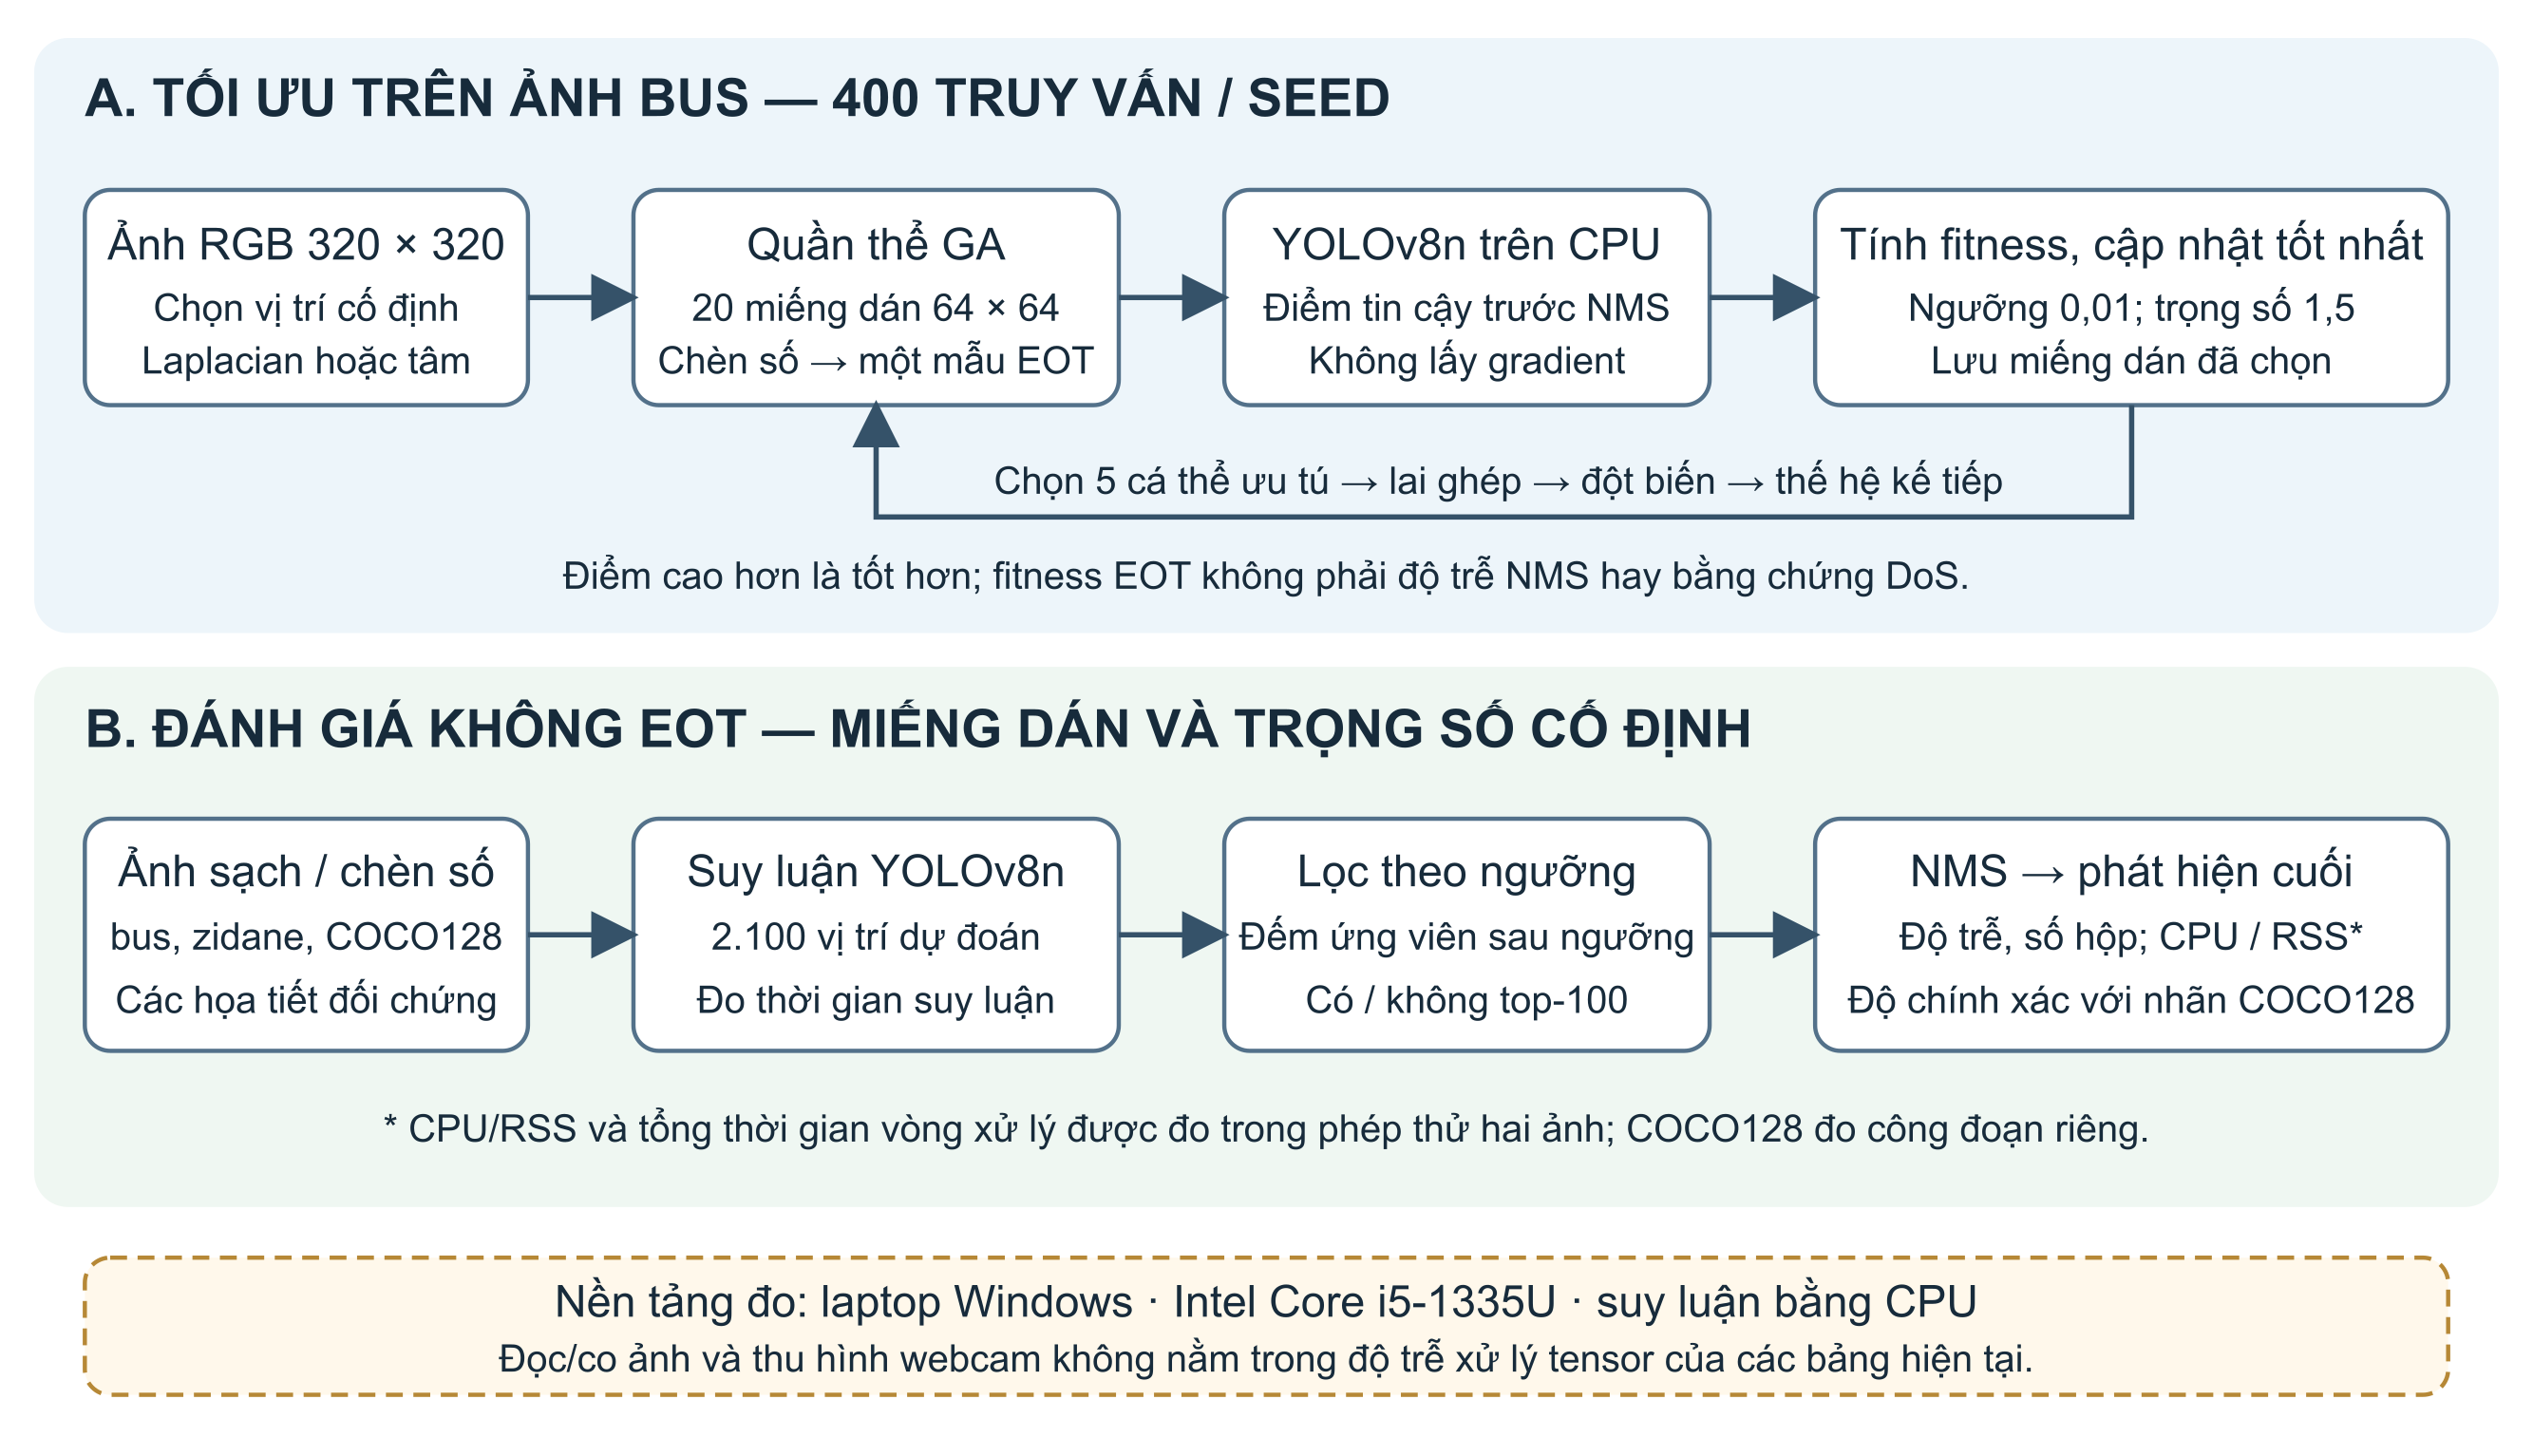
\includegraphics[width=0.98\textwidth]{figures/quy_trinh_kiem_chung_vi.png}
\caption{Kiến trúc Sponge Patch trên laptop: nhánh tối ưu dùng EOT và phản hồi điểm trước NMS; nhánh đánh giá giữ miếng dán cố định, áp dụng ngưỡng và giới hạn ứng viên rồi đo công đoạn. Thời gian xử lý ảnh không bao gồm thu hình webcam.}
\label{fig:pipeline}
\end{figure*}

\subsection{Ký hiệu}

Gọi $x\in[0,1]^{H\times W\times3}$ là ảnh sạch, $p\in[0,1]^{h\times w\times3}$ là miếng dán, $l$ là vị trí, và $A(x,p,l)$ là toán tử chèn miếng dán. Mô hình phát hiện $f_\theta$ sinh tập dự đoán thô
\[
B_{\mathrm{raw}}(x)=\{(b_i,C_i,\hat{y}_i)\}_{i=1}^{K}.
\]
Với ngưỡng tin cậy $\tau$, tập ứng viên đi vào NMS là
\[
B_\tau(x)=\{(b_i,C_i,\hat{y}_i)\in B_{\mathrm{raw}}(x):C_i>\tau\},
\]
Số ứng viên hoạt động là $N_{\mathrm{active}}(x)=|B_\tau(x)|$.
Đầu ra cuối là $D(x)=\mathrm{NMS}(B_\tau(x))$.

Định nghĩa trên mô tả nhánh không giới hạn ứng viên. Với phòng thủ top-$k$, NMS nhận tập $\operatorname{Top}_k(B_\tau)$ theo điểm tin cậy; số đầu vào NMS bằng $\min(N_{\mathrm{active}},k)$. Trong mọi bảng, số ứng viên sau ngưỡng được đếm trước giới hạn này và không bị đổi tên thành số dự đoán thô hay số phát hiện cuối.

\subsection{Cơ sở toán học của Non-Maximum Suppression}

Trong mô hình so sánh mọi cặp, số cặp tiềm năng là
\[
P(N)=\binom{N}{2}=\frac{N(N-1)}{2}.
\]
Với $N=50$, $P=1.225$; với $N=3.000$, $P=4.498.500$. Tỷ lệ là
\[
\frac{P(3000)}{P(50)}=3.672{,}24.
\]
Đây là tỷ lệ số cặp lý thuyết, không phải tỷ lệ độ trễ. NMS xử lý theo lô hoặc vector, loại bỏ sớm, lọc theo lớp, top-$k$, bố trí bộ nhớ và phần cứng có thể làm đường cong thời gian thực thi khác xa $N^2$.

\subsection{Chọn vị trí dựa trên độ nổi bật của ảnh}

Mã triển khai hiện tại không dùng gradient mô hình. Ảnh được chuyển sang ảnh mức xám, sau đó đo đáp ứng Laplacian trên các vùng có kích thước miếng dán. Vị trí $l^*$ có phương sai Laplacian lớn nhất được chọn và giữ cố định trong một lượt chạy:
\[
l^*=\arg\max_l \operatorname{Var}\!\left(\nabla^2 x\big|_l\right).
\]
Thuật toán này là quy tắc kinh nghiệm dựa trên cấu trúc ảnh; nó không chứng minh rằng vị trí được chọn là vị trí nhạy nhất của mô hình phát hiện.

\subsection{Hàm fitness và chiều tối ưu}

Với ảnh đối kháng $x_{\mathrm{adv}}=A(x,p,l^*)$, fitness là
\[
\begin{aligned}
F(p;x)={}&\sum_{i=1}^{K}C_i(x_{\mathrm{adv}})
\mathbf{1}\big[C_i(x_{\mathrm{adv}})>\tau_{\mathrm{opt}}\big]\\
&+\lambda N_{\mathrm{active}}(x_{\mathrm{adv}}).
\end{aligned}
\]
Thuật toán giải
\[
p^*=\arg\max_{p\in[0,1]^{h\times w\times3}}
\mathbb{E}_{t\sim\mathcal{T}}\left[F_t(p;x)\right].
\]
Ở đây $F_t(p;x)$ dùng cùng công thức fitness, nhưng đọc điểm dự đoán trên $t(A(x,p,l^*))$: phép biến đổi tác động lên toàn ảnh sau khi chèn miếng dán. Mã hiện lấy một mẫu EOT mỗi truy vấn; cực đại điểm quan sát không phải ước lượng độc lập, chính xác của kỳ vọng EOT.
Mã nguồn sử dụng $\tau_{\mathrm{opt}}=0{,}01$ và $\lambda=1{,}5$. Ngưỡng này dùng để dẫn hướng tối ưu, không được coi mặc định là ngưỡng triển khai.

\subsection{Thuật toán tiến hóa Sponge Patch}

Mỗi cá thể là tensor RGB $3\times h\times w$. Quần thể khởi tạo từ phân phối đều trên $[0,1]$. Mỗi thế hệ đánh giá fitness theo lô ảnh, giữ $k$ cá thể ưu tú có điểm lớn nhất, lai ghép bằng cắt ngang theo cấu hình mặc định, và đột biến một tỷ lệ cá thể bằng nhiễu đều có biên độ đặt trước. Dừng sớm được kích hoạt khi fitness tốt nhất đã quan sát không tăng quá $\delta$ trong số thế hệ chờ.

Trong các lượt chạy nhiều seed được lưu trước đây, cấu hình chính là miếng dán $64\times64$, ảnh $320\times320$, quần thể 20, tối đa 30 thế hệ, cá thể ưu tú $k=5$, tỷ lệ đột biến 0,1, biên độ đột biến 0,2, số thế hệ chờ 10 và $\delta=0,5$. Miếng dán chiếm
\[
\rho=\frac{64\times64}{320\times320}=4\%.
\]

\begin{algorithm}[t]
\caption{Tối ưu miếng dán bằng GA}
\label{alg:ga}
\begin{algorithmic}[1]
\Require Ảnh $x$, vị trí $l$, quần thể $P$, thế hệ $G$.
\Ensure Miếng dán có fitness quan sát cao nhất $p^*$.
\State Khởi tạo $P$ miếng dán RGB từ phân phối đều.
\State Chọn $l$ bằng phương sai Laplacian hoặc tâm ảnh.
\For{$g=1,\ldots,G$}
\State Chèn từng miếng dán vào ảnh tại $l$.
\State Lấy một mẫu EOT cho mỗi ảnh đã chèn.
\State Đọc điểm trước NMS và tính fitness.
\State Cập nhật $p^*$ nếu fitness quan sát tăng.
\State Giữ 5 cá thể ưu tú; lai ghép bằng cắt ngang.
\State Đột biến với xác suất 0,1, biên độ 0,2.
\EndFor
\State Trả $p^*$; đo lại độc lập trên ảnh gốc và ảnh khác.
\end{algorithmic}
\end{algorithm}

Hình~\ref{fig:ga_flow} cụ thể hóa Thuật toán~\ref{alg:ga} với cấu hình của lượt kiểm chứng hai ảnh ban đầu: 20 cá thể, 20 thế hệ và 400 truy vấn. Lưu đồ chỉ mô tả hai nhánh GA; tìm kiếm ngẫu nhiên sinh 20 mẫu mới mỗi vòng tại vị trí Laplacian, không giữ nhóm ưu tú, lai ghép hoặc đột biến. Việc sinh quần thể sau lượt đánh giá cuối trong mã GA không tạo thêm truy vấn và không thay miếng dán tốt nhất trả về. Lượt mở rộng tính ngân sách theo số ảnh thực sự qua mô hình; vì mỗi cá thể được đánh giá trên bốn ảnh, 400 truy vấn không còn tương ứng 20 thế hệ.

\begin{figure*}[t]
\centering
\includegraphics[width=0.82\textwidth]{figures/luu_do_ga_vi.png}
\caption{Lưu đồ GA khớp cấu hình thực thi trên máy cục bộ. Vị trí được cố định trước tìm kiếm; xác suất đột biến áp dụng cho từng cá thể con, không phải từng pixel. Cực đại fitness quan sát được lưu riêng với quần thể cuối, sau đó miếng dán được đo lại không EOT.}
\label{fig:ga_flow}
\end{figure*}

\subsection{EOT trong mã triển khai}

Trong cấu hình EOT cơ sở, mỗi ảnh qua mô hình nhận một mẫu biến đổi độc lập sau khi chèn miếng dán: xoay trong biên $\pm15$ độ với xác suất 0,8; dao động độ sáng và độ tương phản 0,2 với xác suất 0,8; làm mờ Gaussian bằng bộ lọc $3\times3$, $\sigma$ trong khoảng 0,1--1,0 với xác suất 0,5; và nhiễu Gaussian cộng có độ lệch chuẩn 0,02. Mã hiện chưa có biến đổi phối cảnh hoặc thay đổi tỷ lệ. Phép đo ứng viên, độ trễ và AP trên ảnh gốc giữ cố định miếng dán đã chọn và không dùng EOT. Lượt kiểm chứng mở rộng còn đo riêng bằng các mẫu EOT mới, độc lập với mẫu tối ưu; phần này được báo tách khỏi kết quả trên ảnh gốc tại Mục~\ref{sec:extended_primary}.

\section{Thực nghiệm và đánh giá}

\subsection{Phân loại bằng chứng trong kho mã nguồn}

Các kết quả lưu trước đây được phân thành bốn nhóm theo nguồn dữ liệu. Các lượt chạy cục bộ mới có bản kê cấu hình riêng và được báo cáo tách biệt:

\begin{enumerate}[leftmargin=*]
    \item \textbf{Kết quả tối ưu trên đầu vào ngẫu nhiên:} nhiều seed, tìm kiếm ngẫu nhiên và thực nghiệm theo kích thước miếng dán.
    \item \textbf{Thực nghiệm phát hiện trên ảnh tổng hợp:} đối chứng họa tiết ngẫu nhiên, quét tham số phòng thủ, chương trình đánh giá chuyển giao và cảnh tổng hợp.
    \item \textbf{Phép đo riêng NMS:} hộp ngẫu nhiên được đưa trực tiếp vào \texttt{torchvision.ops.nms}; đây là đầu vào tổng hợp trực tiếp cho NMS.
    \item \textbf{Nhật ký camera và hệ thống:} CSV có thông số nội bộ nhưng thiếu bản kê cấu hình lượt chạy phần cứng/phần mềm, nên chỉ dùng cho kiểm toán, không dùng để đưa ra kết luận nhân quả.
\end{enumerate}

\subsection{Mô hình và đầu vào}

Các kiến trúc phát hiện có cách sinh và lọc hộp khác nhau. YOLOv3 và SSD thuộc hướng phát hiện một giai đoạn; MobileNetV2 cung cấp khối tích chập nhẹ cho ứng dụng hạn chế tài nguyên \cite{yolov3,mobilenetv2,ssd2015}. Faster R-CNN dùng mạng đề xuất vùng, RetinaNet xử lý bài toán mất cân bằng của dự đoán dày đặc, còn DETR biểu diễn phát hiện bằng dự đoán tập hợp \cite{faster2015,retina2017,detr2020}. Những khác biệt này khiến số dự đoán thô và ranh giới hậu xử lý không thể mặc định giống nhau. Mô hình chính trong các phép đo đã hoàn tất là YOLOv8n từ Ultralytics \cite{yolov8docs}.

Mã bao mô hình tải \texttt{yolov8n.pt} qua Ultralytics và gọi mô hình PyTorch để lấy tensor $[B,84,2100]$ tại đầu vào $320\times320$. Số vị trí dự đoán thực đo là $40^2+20^2+10^2=2.100$; mỗi vị trí chứa bốn tọa độ hộp và 80 xác suất lớp. Con số 8.400 ứng với đầu vào $640\times640$, không áp dụng cho cấu hình 320 của thực nghiệm này. YOLOv8n không dùng hộp neo; thuật ngữ “hộp neo thô” không được dùng cho mô hình này.

Trọng số cục bộ có mã SHA-256 bắt đầu bằng \texttt{f59b3d833e2f}; mã băm đầy đủ được lưu trong bản kê cấu hình để kiểm tra đúng tệp khi tái lập. Tệp khớp bản \texttt{yolov8n.pt} được theo dõi tại commit \texttt{6930b7c} của kho mã nguồn, không được huấn luyện lại trong các phép kiểm chứng này.

\begin{table*}[t]
\centering
\small
\caption{Vai trò các mô hình trong phép kiểm chứng đã hoàn tất. Chuyển giao dùng cùng miếng dán nguồn và ảnh chuẩn bị 320×320; hậu xử lý khác nhau theo mô hình nên chỉ đối chiếu sạch/miếng dán trong từng mô hình.}
\begin{tabularx}{\textwidth}{XXXXcc}
\toprule
Vai trò & Kiến trúc & Đầu vào & Hậu xử lý & Tối ưu & Chuyển giao \\
\midrule
Nguồn và đánh giá cục bộ & YOLOv8n & 320×320 & NMS thuần PyTorch, không phân biệt lớp & Có & Nguồn \\
Mô hình đích & YOLOv8s & 320×320 & Cùng mã NMS với nguồn & Không & Có \\
Mô hình đích & SSDLite320 MobileNetV3-Large & 320×320 & Chuẩn hóa và NMS torchvision & Không & Có \\
Mô hình đích & Faster R-CNN MobileNetV3-Large-FPN & Co ảnh nội bộ đặt về 320 & NMS đề xuất vùng và phát hiện & Không & Có \\
Mô hình đích & RetinaNet ResNet50-FPN & Co ảnh nội bộ đặt về 320 & Chuẩn hóa và NMS torchvision & Không & Có \\
Đích không NMS & DETR-ResNet50 & 320×320, chuẩn hóa ImageNet & Dự đoán tập hợp, lọc điểm & Không & Có \\
\bottomrule
\end{tabularx}
\label{tab:model_roles}
\end{table*}

\subsection{Phần cứng và phần mềm}

Các tệp \texttt{requirements.txt} chỉ quy định phiên bản tối thiểu; chúng không xác định đầy đủ môi trường của các nhật ký cũ. Lượt kiểm chứng ngày 02/10/2026 chạy trực tiếp trên Windows 11 Pro, bản hệ điều hành 10.0.26300, CPU Intel Core i5-1335U với 10 nhân và 12 bộ xử lý logic. Tổng RAM hệ thống báo 16.791.998.464 byte, tương đương khoảng 15,64 GiB. PyTorch được giới hạn ở hai luồng tính toán và một luồng liên tác vụ; suy luận dùng CPU, số thực 32 bit. Cấu hình này là máy tính xách tay được giới hạn luồng, không phải phép mô phỏng phần cứng Raspberry Pi hay một máy chủ biên khác.

Phiên bản đang thực thi là Python 3.14.6, PyTorch 2.13.0+cpu, torchvision 0.28.0+cpu, Ultralytics 8.4.90, OpenCV 5.0.0, NumPy 2.5.0, Kornia 0.8.3 và psutil 7.2.2. Bản kê cấu hình lưu đường dẫn trình thông dịch, thời điểm UTC, mã commit Git, mã băm chương trình thực nghiệm, mã nguồn, ảnh và trọng số. Phiên bản được đọc từ mô-đun đang nạp; siêu dữ liệu gói cài đặt cũng được lưu riêng vì torchvision trên máy có thông tin phiên bản gói không trùng phiên bản mô-đun.

\subsection{Thiết bị thu hình và ranh giới đo trên laptop}

Thiết bị thu hình được tác giả xác nhận là webcam ngoài, độ phân giải 720p. Chưa có phép đo FPS thực hoặc cấu hình bộ mã hóa để gắn với những nhật ký cũ. Các bảng mới dưới đây được tạo từ ảnh số trên laptop, không từ phép thử miếng dán đã in qua webcam. Không sử dụng mô tả camera IP, Wi-Fi và MJPEG trong bản gốc làm cấu hình đã xác nhận.

Ảnh được đọc, chuyển sang RGB, co về 320×320 và chuẩn hóa trước khi đo suy luận. Miếng dán được chèn vào tensor đã chuẩn bị. Phép đo tách suy luận, lọc theo điểm tin cậy và NMS; thời gian thu hình, đọc ảnh, giải mã và hiển thị không nằm trong độ trễ này. CPU được tính cho tiến trình thực nghiệm; RSS là bộ nhớ tiến trình, không phải lượng bộ nhớ riêng do miếng dán gây ra. Khi không đọc được nhiệt độ trên Windows, giá trị được xem là không có dữ liệu, không thay bằng 0.

\subsection{Đơn vị thống kê}

Seed của thuật toán tối ưu, khung hình liên tiếp và truy vấn độ trễ lặp lại là ba đơn vị khác nhau. Các kết quả cũ có 10 seed nhưng mỗi seed tối ưu trên một tensor ngẫu nhiên; khung hình liên tiếp không được xem là lượt thực nghiệm độc lập. Phép kiểm chứng cục bộ mới dùng seed 0--9 trên cùng ảnh tối ưu. Mỗi điều kiện đo có ba lượt khởi động và năm lượt đo liên tiếp; trung vị của năm lượt là một quan sát ở mức seed. Trung bình và độ lệch chuẩn mẫu được tính trên 10 quan sát seed; các lần đo lặp không làm tăng số seed.

Phân tích bổ sung lấy mẫu lại ghép cặp 10.000 lần với seed 20261002, tính khoảng tin cậy phân vị 95\% cho trung bình chênh lệch. Với hai ảnh, đơn vị lấy mẫu là cặp seed; với COCO128 là cặp ảnh, điều kiện trên một miếng dán seed 0 cố định. Đây là phân tích thăm dò hậu nghiệm, chưa điều chỉnh nhiều so sánh, không phải kiểm định xác nhận được đăng ký trước. Không suy ra khoảng tin cậy AP từ trung bình AP từng ảnh và không gộp seed với ảnh thành cỡ mẫu chung.

Lượt mở rộng COCO val2017 dùng thiết kế riêng, mô tả tại Mục~\ref{sec:extended_primary}. Đơn vị phân tích chính là seed tối ưu: tỷ số ứng viên được tính trên cùng 128 ảnh trong từng seed trước khi lấy trung bình giữa 10 seed. Khoảng tin cậy dùng 20.000 mẫu bootstrap ghép cặp, không trộn với phân tích hậu nghiệm hai ảnh hoặc COCO128. Các khoảng này điều kiện trên bộ ảnh, mô hình và laptop đã chọn, không phải khoảng tin cậy cho toàn bộ phân bố ảnh tự nhiên.


\subsection{Quy trình kiểm chứng cục bộ}

Hai ảnh ví dụ \texttt{bus.jpg} và \texttt{zidane.jpg} đi kèm Ultralytics được dùng lần lượt để tối ưu và kiểm tra trên ảnh khác. Ảnh RGB được co trực tiếp về $320\times320$ bằng nội suy song tuyến tính, không chèn viền giữ tỷ lệ. Tất cả phương pháp dùng miếng dán $64\times64$, ngân sách 400 truy vấn ảnh mỗi seed, 20 cá thể hoặc mẫu mỗi vòng và 20 vòng. GA giữ 5 cá thể ưu tú, lai ghép cắt ngang, đột biến với xác suất 0,1 và biên độ 0,2; dừng sớm được tắt để giữ ngân sách bằng nhau. Cả ba phương pháp dùng cùng hàm fitness và một mẫu EOT mỗi truy vấn. GA trung tâm cố định vị trí ở $(128,128)$; SG-GA và tìm kiếm ngẫu nhiên dùng vị trí Laplacian $(112,240)$ trên ảnh tối ưu. Vị trí được giữ nguyên khi chuyển sang ảnh kiểm tra.

Thứ tự phương pháp và điều kiện đo được xáo trộn theo seed. Đối chứng gồm ảnh sạch, nhiễu đều, sọc chéo định kỳ và màu xám đặc cùng diện tích. Họa tiết sọc dùng công thức $(\lfloor(r+c)/4\rfloor\bmod2)$ theo hàng $r$, cột $c$; trường \texttt{checkerboard} trong dữ liệu thô của lượt hai ảnh mang tên chưa chính xác và được ghi lại đúng là sọc chéo trong hình công bố. Ngưỡng đánh giá là 0,01 và 0,25; nhánh phòng thủ dùng ngưỡng 0,01 với top-100 trước NMS. Mọi nhánh đều dùng IoU NMS 0,45 và tối đa 300 phát hiện sau NMS. Độ trễ được đo bằng đồng hồ đơn điệu độ phân giải cao, tách suy luận, lọc, NMS và tổng thời gian. RSS đo từ tiến trình thực nghiệm, không được gọi là bộ nhớ tăng do miếng dán khi chưa trừ mức nền.

Tổng thời gian ở phép thử hai ảnh chỉ gồm suy luận, lọc và NMS trên tensor đã chuẩn bị; không gồm đọc/co ảnh, thu hình, truyền mạng hoặc hiển thị. Thông lượng được tính từ số lượt xử lý chia cho thời gian thực của vòng đo, không từ nghịch đảo của trung vị độ trễ. Thời gian tối ưu không tính nạp mô hình và khởi tạo quần thể.

Trên ảnh tối ưu, các họa tiết đối chứng cùng vị trí với SG-GA. Trên ảnh \texttt{zidane}, vị trí họa tiết đối chứng được chọn lại bằng Laplacian, còn ba miếng dán tối ưu giữ vị trí từ \texttt{bus}. Vì vậy, so sánh họa tiết trên ảnh này chịu ảnh hưởng đồng thời của nội dung và vị trí; phép đánh giá COCO128 bổ sung giữ vị trí cố định để tránh sự khác biệt này.

\begin{figure*}[t]
\centering
\includegraphics[width=0.88\textwidth]{outputs/local_q1_20261002_v2/image_examples.png}
\caption{Ảnh đầu vào của phép kiểm chứng cục bộ: ảnh tối ưu sạch, ảnh chèn miếng dán SG-GA seed 0 và ảnh kiểm tra khác nội dung. Miếng dán có kích thước 64×64 trên ảnh 320×320 (4\% diện tích); không vẽ hộp phát hiện trong hình này. Hai ảnh nguồn là ảnh ví dụ đi kèm Ultralytics; đây là chèn số, không phải miếng dán đã in.}
\label{fig:examples}
\end{figure*}

Hình~\ref{fig:examples} minh họa đúng ảnh được đưa vào mô hình sau co kích thước; ảnh kiểm tra không được dùng để tiến hóa miếng dán.

Phép đo riêng NMS dùng 10 seed sinh hộp khác nhau cho mỗi mức $N$, năm lượt khởi động và 20 lượt đo trên cùng bộ hộp. Trung vị 20 lượt tạo một quan sát seed. Kích thước hộp và mức chồng lấn cũng ảnh hưởng thời gian; các điểm $N=3.000$ hoặc 8.400 là tải tổng hợp trực tiếp, không phải số dự đoán của mô hình 320.

\subsection{Kiểm chứng bổ sung trên dữ liệu có nhãn}

COCO (Common Objects in Context) là bộ ảnh những cảnh thường ngày, có nhãn vật thể và vị trí của chúng \cite{coco2014}. Nhãn cho phép kiểm tra cả phát hiện đúng lẫn bỏ sót, thay vì chỉ đếm số hộp do mô hình tạo ra. COCO128 là tập con nhỏ do Ultralytics phân phối để kiểm tra quy trình \cite{coco128}; nó không phải một tập kiểm tra mới độc lập với dữ liệu huấn luyện mô hình.

COCO128 gồm 128 ảnh đầu của COCO train2017 và nhãn hộp định dạng YOLO, tải từ nguồn Ultralytics \cite{coco128}. Tập này có thể trùng dữ liệu huấn luyện của trọng số; nó chỉ được dùng để chẩn đoán hậu xử lý và đánh đổi phòng thủ, không để xác lập khả năng khái quát trên tập kiểm tra độc lập. Miếng dán seed 0 được quy định trước, không chọn theo kết quả COCO128 và không tối ưu lại trên tập này. Ba phương pháp và các họa tiết đối chứng giữ vị trí từ ảnh tối ưu; ảnh sạch là đối chứng ghép cặp theo ảnh.

Phép kiểm chứng này bổ sung ô bàn cờ đúng nghĩa với ô 4×4 pixel, bên cạnh sọc chéo của lượt hai ảnh, nhiễu đều và màu xám. Tổng cộng có tám điều kiện và ba cấu hình hậu xử lý. Kiểm tra trực tiếp tệp ZIP nguồn ghi nhận ảnh 250 và 508 không có tệp nhãn; nhãn 656 và 659 không có ảnh tương ứng. Cả 128 ảnh được giữ lại; hai ảnh thiếu nhãn được xử lý với tập nhãn rỗng theo quy ước của mã nạp Ultralytics, không tự bổ sung nhãn. Bản kê cấu hình lưu danh mục ngoại lệ này; AP là giá trị chẩn đoán phụ thuộc bộ nhãn đã cung cấp.

Mỗi điều kiện trên từng ảnh có một lượt suy luận khởi động và ba lượt đo. Dự đoán được lưu đệm để so sánh ba cấu hình ngưỡng/giới hạn trên cùng đầu ra. Mỗi cấu hình hậu xử lý có hai lượt khởi động và năm lượt đo; trung vị thời gian là quan sát ở mức ảnh. Suy luận và hậu xử lý được đo riêng nên không suy ra FPS toàn trình bằng cách cộng các trung vị. Thứ tự điều kiện và cấu hình được xáo trộn; mọi điều kiện dùng cùng bộ ảnh, kích thước, NMS và trọng số.

Độ chính xác và độ bao phủ được tính gộp các hộp tại IoU 0,5, ghép hộp dự đoán theo điểm giảm dần với hộp nhãn cùng lớp, mỗi nhãn chỉ ghép một lần. AP chẩn đoán dùng nội suy 101 mức độ bao phủ và trung bình các lớp có nhãn; mAP chẩn đoán tiếp tục lấy trung bình tại IoU từ 0,50 đến 0,95, bước 0,05. Đây không phải mAP COCO chính thức: bộ nhãn không có thông tin đối tượng đám đông/bỏ qua, phép ghép và NMS không phải trình đánh giá COCO chuẩn, và AP phụ thuộc ngưỡng lọc được báo. Bốn kiểm tra đơn vị xác nhận hộp khớp chính xác, sai lớp, phát hiện giả đứng trước hộp đúng và hộp trùng lặp.

\subsection{Kiểm chứng chiều fitness}

Mã nguồn dùng \texttt{max}, \texttt{argmax} và \texttt{topk}, do đó fitness càng lớn càng tốt. Điều này phù hợp với phương trình trong mục Hàm fitness và chiều tối ưu. Bất kỳ bảng nào coi số fitness nhỏ hơn là tốt hơn đều sai và đã bị loại.

\subsection{Đo riêng thành phần NMS}

\begin{table}[ht]
\centering
\small
\caption{NMS torchvision đo trực tiếp trên máy cục bộ. Giá trị là trung bình ± độ lệch chuẩn giữa 10 seed hộp; mỗi seed dùng trung vị 20 lượt sau 5 lượt khởi động. Hộp được sinh trực tiếp, không phải đầu ra của mô hình phát hiện.}
\begin{tabular}{rrr}
\toprule
$N$ & Số cặp lý thuyết & Độ trễ (ms) \\
\midrule
50 & 1.225 & $0{,}071\pm0{,}052$ \\
100 & 4.950 & $0{,}064\pm0{,}044$ \\
500 & 124.750 & $0{,}550\pm0{,}354$ \\
1.000 & 499.500 & $1{,}838\pm0{,}582$ \\
2.100 & 2.203.950 & $5{,}514\pm2{,}758$ \\
3.000 & 4.498.500 & $9{,}953\pm2{,}752$ \\
8.400 & 35.275.800 & $70{,}363\pm15{,}055$ \\
\bottomrule
\end{tabular}
\label{tab:nmsbench}
\end{table}

Từ 50 lên 3.000 hộp, số cặp lý thuyết tăng $3.672{,}24\times$, trong khi tỷ lệ hai độ trễ trung bình khoảng $141{,}1\times$. Đây là tỷ số hai trung bình, không phải trung bình tỷ số ghép cặp. Mức 50 và 100 hộp không tăng đơn điệu do thời gian quá ngắn và độ phân tán lớn. Bảng~\ref{tab:nmsbench} và Hình~\ref{fig:nms} mô tả triển khai torchvision trên một máy; chúng không xác lập độ trễ của mã NMS thuần PyTorch trong đường ống phát hiện hay một máy chủ biên khác. Phép đo cũ 0,415/23,647 ms không có bản kê cấu hình nên không được gộp vào kết quả mới.

\begin{figure*}[t]
\centering
\includegraphics[width=0.72\textwidth]{outputs/local_q1_20261002_v2/figures_corrected/nms_local.png}
\caption{Độ trễ NMS torchvision theo số hộp tổng hợp trên CPU i5-1335U. Điểm và thanh sai số là trung bình và độ lệch chuẩn của trung vị thời gian giữa 10 seed hộp. Các mức 3.000 và 8.400 không phải số ứng viên do miếng dán tạo ra.}
\label{fig:nms}
\end{figure*}

\subsection{So sánh tối ưu cùng ngân sách trên ảnh tự nhiên}

\begin{table*}[t]
\centering
\caption{Kết quả tối ưu trên ảnh bus, 10 seed, cùng 400 truy vấn ảnh mỗi seed. Giá trị là trung bình ± độ lệch chuẩn giữa seed. Fitness là cực đại điểm EOT đã quan sát, không phải kỳ vọng EOT được kiểm tra độc lập.}
\begin{tabularx}{\textwidth}{Xrrr}
\toprule
Phương pháp & Fitness tốt nhất & Truy vấn/seed & Thời gian tối ưu (s) \\
\midrule
GA vị trí nổi bật & $312{,}61\pm10{,}65$ & 400 & $81{,}84\pm28{,}41$ \\
GA vị trí trung tâm & $367{,}39\pm18{,}40$ & 400 & $95{,}12\pm26{,}03$ \\
Tìm kiếm ngẫu nhiên & $309{,}97\pm5{,}65$ & 400 & $92{,}09\pm33{,}82$ \\
\bottomrule
\end{tabularx}
\label{tab:optimizer_local}
\end{table*}

Bảng~\ref{tab:optimizer_local} cho thấy GA trung tâm đạt điểm cao hơn SG-GA trong cấu hình này. Chênh lệch SG-GA với tìm kiếm ngẫu nhiên chỉ khoảng 2,64 điểm; chưa có bằng chứng để coi quy tắc Laplacian là lựa chọn vị trí vượt trội. Hình~\ref{fig:convergence} thể hiện cực đại tích lũy theo truy vấn; đường tăng không tự chứng minh miếng dán gây tải cao hơn ảnh sạch vì điểm còn phụ thuộc biến đổi EOT của toàn ảnh.

Chênh lệch fitness ghép cặp SG-GA trừ GA trung tâm là $-54{,}78$, khoảng tin cậy thăm dò 95\% $[-66{,}81;-42{,}45]$. So với tìm kiếm ngẫu nhiên, chênh lệch là $2{,}64$, khoảng $[-1{,}92;7{,}64]$. Kết quả này chỉ mô tả 10 seed trên một ảnh tối ưu, không cho phép xếp hạng phương pháp trên một phân bố ảnh hay phần cứng khác.

\begin{figure*}[t]
\centering
\includegraphics[width=0.72\textwidth]{outputs/local_q1_20261002_v2/figures_corrected/convergence_local.png}
\caption{Tiến trình tìm kiếm trên ảnh bus với cùng ngân sách 400 truy vấn. Đường là trung bình cực đại fitness EOT đã quan sát của 10 seed; vùng mờ là ± một độ lệch chuẩn giữa seed, không phải khoảng tin cậy. Mọi phương pháp đều tối đa hóa fitness.}
\label{fig:convergence}
\end{figure*}

\subsection{Ứng viên và chi phí thực thi trên hai ảnh tự nhiên}

\begin{table*}[t]
\centering
\small
\caption{Đánh giá không EOT tại ngưỡng 0,01, không giới hạn trước NMS. Trung bình ± độ lệch chuẩn giữa 10 seed; mỗi seed dùng trung vị năm lượt đo. Tổng thời gian chỉ gồm suy luận, lọc và NMS. Thông lượng là vòng xử lý ảnh tĩnh, không phải FPS camera.}
\begin{tabularx}{\textwidth}{Xlrrrrr}
\toprule
Điều kiện & Ảnh & Ứng viên & Phát hiện cuối & NMS (ms) & Tổng (ms) & Thông lượng (ảnh/s) \\
\midrule
Sạch & bus & 118,0 & 20,0 & $17{,}82\pm7{,}20$ & $267{,}4\pm122{,}5$ & $4{,}19\pm1{,}53$ \\
SG-GA & bus & $115{,}4\pm4{,}8$ & $20{,}0\pm1{,}1$ & $23{,}30\pm12{,}87$ & $316{,}1\pm164{,}6$ & $3{,}63\pm1{,}86$ \\
GA trung tâm & bus & $134{,}8\pm2{,}7$ & $23{,}4\pm1{,}3$ & $20{,}64\pm6{,}46$ & $268{,}8\pm101{,}1$ & $4{,}03\pm1{,}41$ \\
Sạch & zidane & 122,0 & 20,0 & $18{,}30\pm5{,}84$ & $251{,}6\pm69{,}0$ & $4{,}21\pm1{,}25$ \\
SG-GA & zidane & $119{,}1\pm3{,}5$ & $17{,}7\pm1{,}1$ & $14{,}45\pm5{,}96$ & $242{,}0\pm97{,}7$ & $4{,}46\pm1{,}26$ \\
GA trung tâm & zidane & $135{,}9\pm6{,}9$ & $21{,}1\pm0{,}7$ & $21{,}97\pm9{,}90$ & $285{,}5\pm120{,}5$ & $3{,}81\pm1{,}48$ \\
\bottomrule
\end{tabularx}
\label{tab:pipeline_local}
\end{table*}

SG-GA không khuếch đại số ứng viên ở ngưỡng 0,01 trên cả hai ảnh (Bảng~\ref{tab:pipeline_local}). Tỷ số độ trễ NMS trung bình so với ảnh sạch là khoảng 1,31 trên bus nhưng 0,79 trên zidane; tỷ số tổng thời gian tương ứng là 1,18 và 0,96. Độ phân tán thời gian lớn, nên không quy toàn bộ chênh lệch cho miếng dán. Mức CPU tiến trình chuẩn hóa toàn máy của ảnh sạch và SG-GA trên bus là $12{,}23\pm2{,}81$\% và $11{,}46\pm4{,}86$\%; trên zidane là $12{,}73\pm2{,}59$\% và $12{,}89\pm2{,}67$\%. Các giá trị này không cho thấy cạn kiệt CPU. RSS biến thiên lớn theo thời điểm đo và không được dùng để khẳng định rò rỉ hay cạn kiệt bộ nhớ.

\begin{figure*}[t]
\centering
\includegraphics[width=0.95\textwidth]{outputs/local_q1_20261002_v2/figures_corrected/candidates_latency_bus.png}
\caption{Ứng viên sau ngưỡng và độ trễ NMS thuần PyTorch trên ảnh bus, không giới hạn trước NMS, tại hai ngưỡng đánh giá. Cột và thanh sai số là trung bình ± độ lệch chuẩn giữa 10 seed. Nhiễu và các họa tiết là đối chứng cùng diện tích; sọc chéo là tên đúng của trường checkerboard trong dữ liệu thô.}
\label{fig:bus}
\end{figure*}

\begin{figure*}[t]
\centering
\includegraphics[width=0.95\textwidth]{outputs/local_q1_20261002_v2/figures_corrected/candidates_latency_zidane.png}
\caption{Ứng viên sau ngưỡng và độ trễ NMS trên ảnh zidane, không dùng ảnh này để tối ưu miếng dán. Cột và thanh sai số là trung bình ± độ lệch chuẩn giữa 10 seed. Các miếng dán tối ưu giữ vị trí từ bus; họa tiết đối chứng được chọn lại vị trí Laplacian, nên so sánh họa tiết ở đây có yếu tố nhiễu do vị trí.}
\label{fig:zidane}
\end{figure*}

Hình~\ref{fig:bus} và Hình~\ref{fig:zidane} cho thấy ngưỡng 0,25 làm số ứng viên giảm mạnh ở mọi điều kiện. Trên bus, SG-GA có $42{,}3\pm0{,}9$ ứng viên so với 41 của ảnh sạch; trên zidane, cả hai có 21 ứng viên. Việc tăng nhẹ ứng viên trên một ảnh không xác lập suy giảm dịch vụ; chưa có thời hạn hay tiêu chí thành công DoS được thiết kế trước. Độ chính xác của giới hạn ứng viên cần đánh giá trên dữ liệu có nhãn.

Ở ngưỡng 0,01, khoảng tin cậy thăm dò 95\% của chênh lệch tổng thời gian SG-GA trừ ảnh sạch là $[-34{,}43;154{,}16]$ ms trên bus và $[-56{,}35;30{,}89]$ ms trên zidane. Cả hai đều bao gồm không; không có bằng chứng nhất quán về tăng thời gian toàn vòng xử lý. Đây không phải bằng chứng tương đương hai điều kiện hay bảo đảm hệ thống miễn nhiễm.

\subsection{Ứng viên và độ chính xác trên COCO128}

Phép chạy hoàn tất 3.072 bản ghi, trên 128 ảnh, tám điều kiện và ba cấu hình. Bộ nhãn dùng 929 hộp thuộc 71 lớp. Tại ngưỡng 0,01 không giới hạn trước NMS, SG-GA seed 0 có trung bình 114,78 ứng viên so với 116,06 của ảnh sạch; chênh lệch ghép cặp là $-1{,}28$, khoảng tin cậy thăm dò 95\% $[-5{,}21;2{,}16]$ ứng viên. Chênh lệch NMS trung bình là $-0{,}452$ ms, khoảng $[-0{,}920;-0{,}031]$ ms; không diễn giải phân tích hậu nghiệm này thành chứng minh phòng thủ phổ quát. Kết quả không hỗ trợ khuếch đại tải NMS bởi miếng dán SG-GA đã chọn trên tập này.

\begin{table*}[t]
\centering
\small
\caption{Khối lượng hậu xử lý trên COCO128, 128 ảnh ghép cặp, miếng dán SG-GA seed 0. Hai cột đếm là trung bình giữa ảnh; thời gian NMS là trung vị [Q1; Q3] của các trung vị năm lượt đo từng ảnh. Ứng viên được đếm trước giới hạn; đầu vào NMS được đếm sau giới hạn.}
\begin{tabularx}{\textwidth}{XXrrX}
\toprule
Điều kiện & Cấu hình & Ứng viên & Vào NMS & NMS (ms) [Q1; Q3] \\
\midrule
Sạch & Ngưỡng 0,01 & 116,06 & 116,06 & 5,12 [2,55; 10,88] \\
Sạch & Ngưỡng 0,25 & 23,27 & 23,27 & 1,19 [0,77; 1,84] \\
Sạch & 0,01 + top-100 & 116,06 & 70,31 & 4,51 [2,38; 6,60] \\
SG-GA & Ngưỡng 0,01 & 114,78 & 114,78 & 5,08 [2,70; 10,77] \\
SG-GA & Ngưỡng 0,25 & 21,74 & 21,74 & 1,17 [0,69; 1,71] \\
SG-GA & 0,01 + top-100 & 114,78 & 72,29 & 4,65 [2,56; 6,63] \\
\bottomrule
\end{tabularx}
\label{tab:coco_latency}
\end{table*}

\begin{table*}[t]
\centering
\small
\caption{Độ chính xác chẩn đoán trên cùng 128 ảnh, 929 hộp nhãn. P/R là độ chính xác/độ bao phủ gộp tại IoU 0,5; AP50/mAP dùng nội suy 101 mức và trung bình lớp tại IoU 0,5/0,5--0,95. Tất cả cột chỉ số dùng \%. Đây không phải kết quả mAP COCO chính thức; ngưỡng lọc và NMS không phân biệt lớp được giữ rõ trong từng hàng.}
\begin{tabularx}{\textwidth}{XXrrrr}
\toprule
Điều kiện & Cấu hình & P (\%) & R (\%) & AP50 (\%) & mAP (\%) \\
\midrule
Sạch & Ngưỡng 0,01 & 22,45 & 55,11 & 46,00 & 32,74 \\
Sạch & Ngưỡng 0,25 & 78,93 & 35,09 & 34,66 & 26,89 \\
Sạch & 0,01 + top-100 & 33,33 & 49,19 & 44,71 & 32,17 \\
SG-GA & Ngưỡng 0,01 & 22,19 & 52,85 & 41,70 & 29,82 \\
SG-GA & Ngưỡng 0,25 & 77,40 & 32,08 & 30,98 & 23,96 \\
SG-GA & 0,01 + top-100 & 31,78 & 47,58 & 40,43 & 29,34 \\
\bottomrule
\end{tabularx}
\label{tab:coco_accuracy}
\end{table*}

Bảng~\ref{tab:coco_latency} và Bảng~\ref{tab:coco_accuracy} phân biệt chi phí hậu xử lý với chất lượng phát hiện. Ở ngưỡng 0,01, AP50 chẩn đoán giảm từ 46,00\% xuống 41,70\% khi chèn SG-GA, trong khi số ứng viên và thời gian NMS không tăng. Điều này là suy giảm tính toàn vẹn của phát hiện trong phép thử, không phải bằng chứng tấn công tính sẵn sàng. Hình~\ref{fig:coco} giữ đầy đủ các phương pháp và họa tiết đối chứng; các miếng dán khác cũng làm giảm độ bao phủ ở mức độ tương tự.

\begin{figure*}[t]
\centering
\includegraphics[width=0.95\textwidth]{outputs/local_coco128_20261002/figures_corrected/accuracy_defense.png}
\caption{Độ bao phủ và AP50 chẩn đoán trên 128 ảnh COCO128 cho tám điều kiện và ba cấu hình hậu xử lý. Các chỉ số có thang 0--1; AP được tính gộp bộ ảnh, không phải trung bình AP từng ảnh. Mỗi phương pháp dùng miếng dán seed 0 cố định và cùng bộ nhãn; không có thanh sai số vì không đánh giá phân bố miếng dán theo seed trong lượt này.}
\label{fig:coco}
\end{figure*}

\subsection{Mở rộng kiểm chứng trên COCO val2017}
\label{sec:extended_primary}

Để kiểm tra kết quả ngoài hai ảnh ví dụ, lượt mở rộng giữ các thành phần chính của Sponge Patch: fitness trước NMS, định vị bằng phương sai Laplacian, tiến hóa nội dung RGB và EOT. Bốn ảnh đầu theo thứ tự ID của COCO128 được dùng để tối ưu; tập kiểm tra gồm 128 ID nhỏ nhất của COCO val2017, được cố định trước khi tối ưu và không trùng bất kỳ ảnh nào của COCO128. Nhãn được lấy nguyên từ tệp COCO gốc, gồm 906 chú thích với thông tin vùng đám đông và bỏ qua, cùng danh mục 80 lớp. Việc tách này bảo đảm tập kiểm tra không dùng để tối ưu miếng dán; lịch sử lựa chọn trọng số YOLOv8n theo dữ liệu xác thực của nhà phát hành chưa được xác định, nên không gọi đây là tập hoàn toàn chưa từng được dùng để lựa chọn mô hình.

Bốn nhánh tìm kiếm gồm SG-GA, GA trung tâm, GA vị trí ngẫu nhiên và tìm kiếm ngẫu nhiên. Mỗi nhánh dùng 10 seed và lưu miếng dán tại 400, 1.000 và 2.500 lượt suy luận ảnh. GA giữ quần thể 20, nhóm ưu tú 5, lai ghép ngang và xác suất đột biến 0,1. Lượt mở rộng dùng nhiễu Gaussian đột biến với độ lệch chuẩn 0,2 rồi chặn về $[0,1]$, khác phép đột biến nhiễu đều của lượt hai ảnh; hai lượt không được gộp thành một thí nghiệm đồng nhất. Vị trí Laplacian được chọn riêng cho mỗi ảnh, có xét cửa sổ ở biên; chính sách này được giữ khi đánh giá, không chọn lại miếng dán theo kết quả kiểm tra. Mỗi đánh giá cá thể dùng bốn ảnh và một mẫu EOT mỗi ảnh, nên tốn bốn truy vấn; cấu hình bốn mẫu EOT tốn 16 truy vấn mỗi cá thể. Dừng sớm bị tắt và ngân sách tính theo lượt ảnh, không theo số lời gọi batch.

Các phép loại bỏ thành phần bổ sung kiểm tra diện tích, từng thành phần EOT và giới hạn ứng viên trong mục tiêu tối ưu; một đối chứng gradient tanh được báo riêng là điều chỉnh cục bộ lấy cảm hứng từ Overload, không phải tái lập nguyên bản hay cùng quyền truy cập với SG-GA. Tổng cộng 16 cấu hình đã hoàn tất 160 lượt tối ưu và 240 checkpoint. Bộ đánh giá đã hoàn tất 250 ca, gồm các checkpoint và 10 đối chứng sạch theo seed. Mức 1.000 truy vấn được đánh giá trên 32 ID đầu; mức 400 và 2.500 dùng đủ 128 ảnh. Không dùng số ảnh khác nhau này để dựng đường cong ngân sách mà không giới hạn về cùng 32 ID. Đánh giá EOT độc lập dùng tám ảnh, 16 mẫu biến đổi ghép cặp mới mỗi ảnh, không tái sử dụng mẫu tối ưu.

Đầu vào vẫn co trực tiếp về $320\times320$. Hậu xử lý chính dùng NMS không phân biệt lớp của mã bao, IoU 0,45 và tối đa 300 phát hiện sau NMS. Lượt đánh giá mở rộng có một lượt khởi động và ba lượt đo suy luận; lọc và NMS được đo riêng trên dự đoán đã lưu, lấy trung vị ba lượt. Đây không phải độ trễ thu hình hoặc tổng độ trễ tính bằng cách cộng hai trung vị. AP được tính gộp trên bộ ảnh bằng \texttt{pycocotools.COCOeval}, với IoU 0,50--0,95, các giới hạn 1/10/100 phát hiện và ID lớp gốc. Kết quả là AP COCO chính thức trên tập con 128 ảnh, không phải kết quả của toàn bộ 5.000 ảnh val2017, cũng không đồng nhất với AP chẩn đoán COCO128 ở trên.

Giả thuyết chính và mức chênh lệch có ý nghĩa thực tiễn được ghi trong giao thức trước phép đánh giá: SG-GA có tỷ số ứng viên cao hơn GA trung tâm ít nhất 0,1 ở ngân sách 2.500. Với seed $s$, đại lượng so sánh là
\[
\begin{aligned}
R_s&=\frac{1}{128}\sum_{i=1}^{128}\frac{N^{\mathrm{patch}}_{i,s}}{\max(1,N^{\mathrm{clean}}_{i,s})},\\
\Delta_s&=R_s^{\mathrm{SG}}-R_s^{\mathrm{center}}.
\end{aligned}
\]
Ngưỡng là 0,01 và không giới hạn ứng viên trước NMS. Mẫu số được chặn tối thiểu bằng 1 theo giao thức để xử lý ảnh sạch không có ứng viên. Phân tích ghép cặp dùng 10 seed, 20.000 mẫu bootstrap và kiểm định đảo dấu hai phía trên đủ $2^{10}=1.024$ cấu hình. Kiểm định dựa trên giả định chênh lệch ghép cặp đối xứng dấu dưới giả thuyết không; đây không phải phép ngẫu nhiên hóa việc gán phương pháp cho ảnh. Giao thức được lưu cục bộ, không phải đăng ký trước trên một cơ sở đăng ký bên ngoài.

\begin{table*}[t]
\centering
\small
\caption{So sánh các phương pháp trên 128 ảnh COCO val2017, ngưỡng 0,01, không giới hạn trước NMS. Bốn phương pháp dùng cùng 2.500 lượt suy luận ảnh, diện tích 4\% và 10 seed; SG-GA so với GA trung tâm là so sánh chính. Tỷ số ứng viên là trung bình ± độ lệch chuẩn giữa seed của $R_s$; AP tính gộp bộ ảnh trong mỗi seed rồi lấy trung bình, đơn vị \%. Thời gian đến checkpoint 2.500 là trung bình ± độ lệch chuẩn giữa 10 lượt tối ưu, không gồm tải mô hình hoặc chọn vị trí.}
\begin{tabularx}{\textwidth}{Xrrrr}
\toprule
Điều kiện & Lượt ảnh/seed & Tỷ số ứng viên & AP hộp (\%) & Tối ưu (s) \\
\midrule
Ảnh sạch & 0 & 1,0000 & 34,08 & -- \\
SG-GA & 2.500 & $1{,}0278\pm0{,}0083$ & 29,97 & $192{,}2\pm28{,}9$ \\
GA trung tâm & 2.500 & $1{,}0329\pm0{,}0093$ & 25,88 & $187{,}6\pm27{,}1$ \\
GA vị trí ngẫu nhiên & 2.500 & $1{,}0519\pm0{,}0092$ & 30,27 & $183{,}3\pm13{,}0$ \\
Tìm kiếm ngẫu nhiên & 2.500 & $1{,}0268\pm0{,}0072$ & 29,93 & $181{,}8\pm8{,}9$ \\
\bottomrule
\end{tabularx}
\label{tab:extended_primary}
\end{table*}

Chênh lệch trung bình SG-GA trừ GA trung tâm là $-0{,}0051$, khoảng bootstrap 95\% $[-0{,}0112;0{,}0007]$, $p=0{,}1504$ ở kiểm định hai phía với giá trị không bằng 0. Khoảng này không hỗ trợ mức ưu thế 0,1 đã đặt ra, nhưng cũng không phải bằng chứng hai phương pháp tương đương. So với ảnh sạch, SG-GA có mức tăng nhẹ theo định nghĩa tỷ số ứng viên; vì vậy, không kéo dài kết luận “không tăng ứng viên” của hai ảnh sang mọi ảnh kiểm tra. AP trung bình giảm từ 34,08\% xuống 29,97\%, cho thấy tác động lên dự đoán ngay cả khi chưa xác lập suy giảm tính sẵn sàng. Mức tăng ứng viên, giảm AP và tăng độ trễ là ba kết quả khác nhau; Bảng~\ref{tab:extended_primary} không đủ để gọi tấn công là DoS.

GA vị trí ngẫu nhiên có tỷ số ứng viên trung bình cao hơn SG-GA trên bộ ảnh cố định này. Chênh lệch SG-GA trừ nhánh vị trí ngẫu nhiên là $-0{,}0241$, khoảng bootstrap 95\% $[-0{,}0315;-0{,}0163]$, với $p$ Holm 0,0293 trong nhóm 15 phép so sánh thứ cấp. Chênh lệch SG-GA trừ tìm kiếm ngẫu nhiên là 0,0010, khoảng $[-0{,}0050;0{,}0073]$ và $p$ Holm 1,0000. Như vậy, chọn vị trí bằng Laplacian chưa đem lại ưu thế theo chỉ tiêu ứng viên trong phép thử này; kết quả không chứng minh mọi cách chọn vị trí ngẫu nhiên đều tốt hơn hoặc khác biệt về độ trễ có cùng chiều.

Hình~\ref{fig:extended_candidates} đặt mức tăng ứng viên của bốn phương pháp trên cùng thang đo. Hiệu ứng trên ảnh kiểm tra nhỏ hơn nhiều so với những tỷ lệ từ hộp tổng hợp hoặc nhiễu toàn ảnh; các đại lượng này không thuộc cùng một phép thử.

\begin{figure*}[t]
\centering
\includegraphics[width=0.92\textwidth]{outputs/extended_q1_20261002/figures/ty_so_ung_vien.png}
\caption{Tỷ số ứng viên của bốn phương pháp trên 128 ảnh val2017, 10 seed, miếng dán 4\% và 2.500 lượt suy luận ảnh. Thanh sai số là khoảng bootstrap 95\% theo seed, điều kiện trên bộ ảnh cố định; không phải độ lệch chuẩn hoặc khoảng cho quần thể ảnh. Đường đứt tại 1 là mức ảnh sạch trong phép thử này. Đây không phải tỷ số độ trễ hay xác nhận DoS.}
\label{fig:extended_candidates}
\end{figure*}

Đồng hồ tối ưu bắt đầu sau khi khởi tạo mô hình, vị trí, quần thể và EOT. Thời gian đến checkpoint gồm vòng tìm kiếm và thao tác lưu miếng dán, không phải tổng thời gian chuẩn bị một cuộc tấn công. Các số trong Bảng~\ref{tab:extended_primary} mô tả những lượt chạy đã thực hiện trên máy cá nhân; không dùng chênh lệch vài giây để khẳng định phương pháp nhanh hơn khi chưa cô lập ảnh hưởng tiến trình nền. Nhật ký 40 lượt của bốn phương pháp ghi đủ 25.000 phép đánh giá cá thể, mỗi cá thể dùng bốn lượt ảnh. Fitness tốt nhất đã quan sát của SG-GA tăng từ 135,72 tại 400 lên 141,50 tại 2.500; mức tăng của một cực đại tích lũy dưới EOT ngẫu nhiên không chứng minh hội tụ hay khả năng khái quát.

Để so ngân sách, Bảng~\ref{tab:extended_budget} chỉ dùng 32 ID kiểm tra chung ở cả ba mốc. Trên tập này, SG-GA không có tỷ số ứng viên tăng đơn điệu theo ngân sách. Kết quả tại 2.500 trên 32 ảnh cũng khác mức 1,0278 trên toàn bộ 128 ảnh, phản ánh phụ thuộc vào bộ nội dung đã chọn. Không so trực tiếp AP của mốc 1.000 trên 32 ảnh với AP của các mốc dùng 128 ảnh, hoặc chọn ngân sách cuối theo kết quả kiểm tra.

\begin{table*}[t]
\centering
\small
\caption{Tỷ số ứng viên so với ảnh sạch trên cùng 32 ID val2017, ngưỡng 0,01, không giới hạn trước NMS và không EOT khi kiểm tra. Mỗi ô là trung bình ± độ lệch chuẩn giữa 10 seed, diện tích miếng dán 4\%. Đây là phân tích mô tả theo ngân sách lượt suy luận ảnh; không phải AP, tỷ số độ trễ hoặc số truy vấn để hội tụ.}
\begin{tabularx}{\textwidth}{Xrrr}
\toprule
Phương pháp & 400 lượt ảnh & 1.000 lượt ảnh & 2.500 lượt ảnh \\
\midrule
SG-GA & $1{,}0004\pm0{,}0110$ & $1{,}0057\pm0{,}0136$ & $0{,}9954\pm0{,}0125$ \\
GA trung tâm & $1{,}0014\pm0{,}0046$ & $1{,}0044\pm0{,}0066$ & $1{,}0109\pm0{,}0093$ \\
GA vị trí ngẫu nhiên & $1{,}0316\pm0{,}0223$ & $1{,}0345\pm0{,}0195$ & $1{,}0353\pm0{,}0224$ \\
Tìm kiếm ngẫu nhiên & $0{,}9947\pm0{,}0089$ & $0{,}9938\pm0{,}0132$ & $0{,}9934\pm0{,}0140$ \\
\bottomrule
\end{tabularx}
\label{tab:extended_budget}
\end{table*}

Hình~\ref{fig:extended_budget} nối ba mốc ngân sách trên đúng bộ ảnh chung của Bảng~\ref{tab:extended_budget}. Đường nối chỉ hỗ trợ đọc xu hướng giữa các mốc đã đo, không biểu diễn số liệu ở những ngân sách trung gian.

\begin{figure*}[t]
\centering
\includegraphics[width=0.92\textwidth]{outputs/extended_q1_20261002/figures/ngan_sach_truy_van.png}
\caption{Ba mốc 400, 1.000 và 2.500 lượt suy luận ảnh trên cùng 32 ID kiểm tra, 10 seed mỗi phương pháp. Vùng mờ là khoảng bootstrap 95\% theo seed, điều kiện trên bộ ảnh cố định, không phải độ lệch chuẩn. Mốc 1 trên trục đứng biểu thị mức ảnh sạch; không dùng đồ thị này để suy ra AP trên 128 ảnh, thời gian hội tụ hay mức tăng độ trễ.}
\label{fig:extended_budget}
\end{figure*}

\subsection{Đối chứng cùng diện tích trên tập kiểm tra có nhãn}

Lượt đối chứng mở rộng đã hoàn tất sáu điều kiện với 10 seed, cùng 128 ảnh val2017, vị trí Laplacian và diện tích 4\%. Nhiễu Gaussian có trung bình 0,5, độ lệch chuẩn 0,25 và được chặn về $[0,1]$; nhiễu đều lấy mẫu trực tiếp trong khoảng này. Họa tiết giống QR là lưới nhị phân ngẫu nhiên 16×16, phóng bằng nội suy láng giềng gần nhất lên 64×64, không phải mã QR hợp lệ. Ô bàn cờ gồm ô 4×4 pixel, màu xám đặc có giá trị 0,5. Hai họa tiết cuối xác định hoàn toàn, nên 10 lượt đo không tạo ra 10 miếng dán độc lập.

Đối chứng gradient giảm độ tin cậy dùng cùng bốn ảnh tối ưu và EOT, với mục tiêu giảm tổng giá trị hàm tanh trên điểm lớp lớn nhất của mỗi vị trí dự đoán. Nó thực hiện 100 bước gradient dấu, bước 1/255, tổng 400 lượt suy luận ảnh và 100 lượt lan truyền ngược; lưu đúng miếng dán đã được đo ở bước cuối. Đây là đối chứng cục bộ nhằm vào dự đoán, không phải tái lập một tấn công tính toàn vẹn đã công bố. Các họa tiết không tối ưu dùng 0 truy vấn, còn SG-GA và gradient dùng 400. So sánh này giữ diện tích và tập ảnh, nhưng không giữ cùng số truy vấn thực dùng giữa họa tiết và các phương pháp tối ưu; quyền gradient của đối chứng cũng khác quyền hộp xám của SG-GA.

\begin{table*}[t]
\centering
\small
\caption{Đối chứng trên cùng 128 ảnh val2017, ngưỡng 0,01, không giới hạn trước NMS, cùng diện tích 4\%. Tỷ số ứng viên tính theo $R_s$; dấu ± là độ lệch chuẩn giữa các miếng dán độc lập. AP hộp COCO tập con tính gộp ảnh trước khi lấy trung bình, đơn vị \%. Ô bàn cờ và màu xám chỉ có một họa tiết, không báo sai số giữa seed như biến thiên tối ưu.}
\begin{tabularx}{\textwidth}{Xrrrr}
\toprule
Điều kiện & Truy vấn tối ưu & Miếng dán độc lập & Tỷ số ứng viên & AP hộp \\
\midrule
Ảnh sạch & 0 & --- & 1,0000 & 34,08 \\
SG-GA & 400 & 10 & $1{,}0303\pm0{,}0059$ & 30,17 \\
Nhiễu đều & 0 & 10 & $1{,}0279\pm0{,}0074$ & 30,08 \\
Nhiễu Gaussian & 0 & 10 & $1{,}0251\pm0{,}0060$ & 30,46 \\
Ô bàn cờ & 0 & 1 & 0,9859 & 31,43 \\
Họa tiết giống QR & 0 & 10 & $1{,}0381\pm0{,}0253$ & 30,21 \\
Màu xám đặc & 0 & 1 & 1,0094 & 31,37 \\
Gradient giảm độ tin cậy & 400 & 10 & $1{,}0092\pm0{,}0071$ & 30,62 \\
\bottomrule
\end{tabularx}
\label{tab:extended_controls}
\end{table*}

Bảng~\ref{tab:extended_controls} cho thấy mức tăng ứng viên của SG-GA 400 gần với nhiễu đều; họa tiết giống QR có trung bình cao hơn nhưng biến thiên giữa miếng dán cũng lớn hơn. Đây là mô tả kết quả, chưa khẳng định chênh lệch có ý nghĩa thống kê. Các họa tiết đơn giản cũng làm AP giảm, nên không quy toàn bộ giảm độ chính xác cho quá trình tối ưu đối kháng. Đối chứng gradient không có AP kiểm tra thấp nhất trong nhóm; tối ưu theo mục tiêu giảm điểm tin cậy không bảo đảm giảm AP mạnh hơn mọi họa tiết. Những quan sát này cho thấy cần giữ đối chứng che khuất và họa tiết không tối ưu khi đánh giá Sponge Patch. Chúng không thay cho phép đo thời gian xử lý hoặc kiểm chứng tấn công tính sẵn sàng.

\subsection{Thời gian xử lý và ảnh hưởng của triển khai NMS}

Để kiểm tra mối nối giữa miếng dán và chi phí thực thi, nghiên cứu đo lại trên 16 ID đầu của tập kiểm tra val2017 đã cố định. Đây là tập con của 128 ảnh, không phải một tập kiểm tra mới được chọn theo hiệu quả tấn công. Mỗi seed sử dụng miếng dán ở ngân sách 2.500 truy vấn của SG-GA, GA trung tâm, GA vị trí ngẫu nhiên và tìm kiếm ngẫu nhiên, cùng ảnh sạch. Ba cấu hình 1, 2 và 4 luồng CPU đều chạy trên một laptop, không được tính thành ba thiết bị. Thứ tự 30 khối seed--cấu hình luồng, điều kiện và ảnh được xáo trộn; mỗi ảnh có một lượt khởi động và ba lần đo.

Một đồng hồ liên tục bao quanh suy luận, giải mã dự đoán, lọc điểm tin cậy và NMS. Đọc ảnh, đặt miếng dán, thu hình và thời gian chờ hàng đợi nằm ngoài ranh giới này. Ngưỡng là 0,01, IoU NMS 0,45, không giới hạn ứng viên trước NMS và giữ tối đa 300 phát hiện đầu ra. Ngân sách xử lý 300 ms được lưu trước phép đo; nó không phải thời hạn từ cảm biến đến kết quả. Trong mỗi khối và điều kiện, trung vị cùng phân vị 95\% được tính từ 48 số đo (16 ảnh × 3 lần); sau đó lấy trung bình giữa 10 khối seed. Ba lần đo lặp không được xem là ba lượt tối ưu độc lập.

\begin{table*}[t]
\centering
\small
\caption{Thời gian xử lý tensor đã chuẩn bị trên cùng laptop, đơn vị ms. Cột trung vị là trung bình ± độ lệch chuẩn của trung vị 10 khối; cột phân vị 95\% là trung bình của phân vị từng khối, không phải phân vị của dữ liệu gộp. Bảng trình bày ảnh sạch và hai GA của so sánh chính. Tỷ lệ vượt ngân sách 300 ms bằng 0 trong cả năm điều kiện, tổng 7.200 số đo.}
\begin{tabularx}{\textwidth}{rXrrr}
\toprule
Luồng CPU & Điều kiện & Trung vị & Phân vị 95\% & Vượt 300 ms (\%) \\
\midrule
1 & Ảnh sạch & $51{,}09\pm1{,}34$ & 78,20 & 0 \\
1 & SG-GA & $52{,}87\pm4{,}41$ & 82,69 & 0 \\
1 & GA trung tâm & $51{,}18\pm0{,}91$ & 74,03 & 0 \\
2 & Ảnh sạch & $78{,}66\pm3{,}68$ & 97,21 & 0 \\
2 & SG-GA & $79{,}32\pm1{,}69$ & 94,11 & 0 \\
2 & GA trung tâm & $79{,}56\pm3{,}04$ & 95,90 & 0 \\
4 & Ảnh sạch & $58{,}83\pm3{,}85$ & 76,21 & 0 \\
4 & SG-GA & $58{,}94\pm1{,}76$ & 78,26 & 0 \\
4 & GA trung tâm & $60{,}19\pm2{,}18$ & 74,14 & 0 \\
\bottomrule
\end{tabularx}
\label{tab:extended_processing}
\end{table*}

Trong Bảng~\ref{tab:extended_processing}, thời gian của SG-GA gần ảnh sạch ở cả ba cấu hình; phân vị 95\% cũng không tăng nhất quán. Không có số đo nào vượt 300 ms, kể cả GA vị trí ngẫu nhiên và tìm kiếm ngẫu nhiên. Kết quả này chưa xác lập suy giảm dịch vụ do miếng dán trong ranh giới đo đã chọn, nhưng không bảo đảm hệ thống camera luôn đáp ứng thời hạn: độ trễ thu hình và hàng đợi chưa nằm trong phép đo. Cấu hình nhiều luồng hơn không luôn nhanh hơn trên máy này; sự khác biệt còn chịu điều phối CPU, tiến trình nền và thứ tự thực thi. Vì vậy, không suy rộng thứ hạng cấu hình sang laptop khác, cũng không đổi nghịch đảo trung vị thành FPS camera.

Ảnh hưởng của mã NMS được kiểm tra riêng bằng dự đoán đã giải mã và lưu từ cùng 16 ảnh, 10 seed, ảnh sạch và SG-GA 2.500. NMS thuần PyTorch trong mã bao và \texttt{torchvision.ops.nms} nhận cùng tensor, cùng lọc ngưỡng, IoU và giới hạn đầu ra; ba cấu hình là ngưỡng 0,01 không giới hạn, ngưỡng 0,25 không giới hạn và ngưỡng 0,01 với top-100. Tổng cộng có 1.920 cấu hình đo, mỗi cấu hình khởi động một lần rồi đo năm lần trên hai luồng CPU. So sánh này chỉ đo phần hậu xử lý, không suy luận lại mô hình.

Ở ngưỡng 0,01 không giới hạn, mỗi ảnh lấy trung vị năm lần đo, mỗi khối seed lấy trung vị của 16 ảnh, rồi lấy trung bình và độ lệch chuẩn giữa 10 khối. Theo cách tổng hợp này, thời gian NMS trên ảnh sạch là $1{,}520\pm0{,}364$ ms với mã thuần PyTorch và $0{,}060\pm0{,}011$ ms với torchvision; các số tương ứng của SG-GA là $1{,}691\pm0{,}129$ và $0{,}062\pm0{,}011$ ms. Đồng hồ NMS trong hàm hậu xử lý gồm cả chọn chỉ số và lấy tối đa 300 phát hiện. Hai cách triển khai trả tensor phát hiện trùng khớp hoàn toàn trong các trường hợp đã kiểm tra, không có nghĩa chúng luôn trùng trong mọi trường hợp bằng điểm hoặc sát ngưỡng IoU. Chênh lệch thời gian cho thấy chi phí NMS phụ thuộc triển khai; không được áp tỷ lệ từ NMS thuần PyTorch sang mã tối ưu. Khớp đầu ra trên bộ tensor cố định cũng không thay cho đánh giá độ chính xác trên phân bố camera.

Các hàng đợi FIFO và bỏ khi bận dựng từ số đo thời gian được giữ riêng như mô hình ngoại tuyến, không dùng để khẳng định điều tiết tải đã được thử qua webcam. Cờ trễ của mô hình này so với chu kỳ phát 100, 200 hoặc 300 ms, khác cờ vượt ngân sách xử lý 300 ms trong bảng. Việc bỏ đầu vào phải được tính vào suy giảm dịch vụ, không chỉ báo tỷ lệ trễ trên phần ảnh còn được xử lý.

\subsection{Luồng xử lý thực và điều tiết đầu vào}
\label{sec:extended_stream}

Để đưa hàng đợi vào ranh giới đo, chương trình phát ảnh theo lịch cố định và một luồng xử lý thực chạy mô hình, giải mã dự đoán, lọc, NMS và chuyển đổi dự đoán sang định dạng COCO. Đây là thực thi đồng thời có mốc thời gian đơn điệu, không phải dựng hàng đợi từ thời gian đã lưu. Đầu vào vẫn là tensor ảnh đã chuẩn bị, không gồm camera, đọc ảnh, đổi kích thước hay chèn miếng dán. Tổng cộng có 240 lượt: 10 seed, hai chu kỳ phát 100/300 ms, bốn điều kiện và ba chính sách. Mỗi lượt phát đúng 32 ảnh val2017 theo cùng thứ tự ghép cặp trong một seed; thứ tự các lượt được xáo trộn. Bốn điều kiện gồm ảnh sạch, SG-GA 400, SG-GA 2.500 và gradient tanh 400, cùng mô hình YOLOv8n, diện tích miếng dán 4\%, hai luồng CPU, ngưỡng 0,01, IoU 0,45 và không giới hạn ứng viên trước NMS. Nhánh 2.500 có ngân sách riêng; nhánh gradient có quyền truy cập mạnh hơn SG-GA. Mỗi lượt khởi động bằng ba ảnh trước khi bắt đầu phát theo lịch.

FIFO nhận toàn bộ đầu vào và cho phép hàng đợi tăng trong lượt hữu hạn này. Chính sách bỏ khi bận chỉ nhận ảnh khi không có ảnh đang xử lý hoặc chờ. Nhánh thích nghi cũng không nhận khi bận, đồng thời đặt khoảng nhận tối thiểu bằng giá trị lớn hơn giữa chu kỳ phát và 1,2 lần trung bình trượt mũ của thời gian xử lý đã hoàn tất, giới hạn trên 600 ms. Hệ số cập nhật trung bình trượt là 0,25; phản hồi chỉ được cập nhật sau khi xử lý xong, không dùng thời gian của ảnh chưa được xử lý.

Thời hạn 300 ms được tính từ mốc phát theo lịch, nên gồm dao động của bộ phát, chờ hàng đợi và xử lý. Chương trình lưu riêng tuổi ảnh từ lúc đến thực tế để không nhầm hai ranh giới. Thông lượng đúng hạn tính số ảnh hoàn tất đúng hạn chia cho khoảng đo; mẫu số không nhỏ hơn 32 chu kỳ phát, kể cả khi lượt hữu hạn kết thúc sớm. Chỉ tiêu này là ảnh/s của luồng phần mềm, không phải FPS webcam. COCOeval giữ toàn bộ 32 ID trong mẫu số: AP toàn luồng coi ảnh bị bỏ là dự đoán rỗng, AP đúng hạn coi cả ảnh bị bỏ và ảnh trễ là dự đoán rỗng.

Tiêu chí lưu trước lượt thử này đánh dấu suy giảm dịch vụ khi thông lượng đúng hạn dưới 80\% tốc độ phát hoặc tỷ lệ thiếu/trễ trên 10\%. Tiêu chí kết hợp còn đòi AP đúng hạn không thấp hơn AP toàn luồng của ảnh sạch FIFO ghép cặp quá hai điểm phần trăm. Không đạt tiêu chí này không tự xác định nguyên nhân là tấn công; ảnh sạch là đối chứng bắt buộc để phân biệt quá tải nền với tác động của miếng dán. Các so sánh chính sách theo seed là thăm dò, không điều chỉnh đa so sánh cho 48 kiểm định được lưu.

\begin{table*}[t]
\centering
\small
\caption{Luồng phần mềm với chu kỳ 100 ms, thời hạn 300 ms, 32 ảnh mỗi lượt và 10 seed mỗi điều kiện/chính sách. Các ô là trung bình ± độ lệch chuẩn giữa lượt chạy; giá trị không đổi chỉ ghi trung bình. “Thiếu/trễ” tính trên toàn bộ ảnh đã phát, gồm ảnh bị bỏ và ảnh hoàn tất sau thời hạn. AP đúng hạn dùng toàn bộ 32 ID, với dự đoán rỗng cho ảnh bị bỏ hoặc trễ; không phải AP chỉ trên các ảnh được xử lý.}
\begin{tabularx}{\textwidth}{XXrrrr}
\toprule
Điều kiện & Chính sách & Được xử lý (\%) & Thiếu/trễ (\%) & Đúng hạn (ảnh/s) & AP đúng hạn (\%) \\
\midrule
Ảnh sạch & FIFO & $100{,}00$ & $85{,}31\pm5{,}90$ & $1{,}08\pm0{,}48$ & $5{,}55\pm2{,}80$ \\
Ảnh sạch & Bỏ khi bận & $49{,}06\pm1{,}51$ & $50{,}94\pm1{,}51$ & $4{,}89\pm0{,}16$ & $19{,}49\pm3{,}21$ \\
Ảnh sạch & Thích nghi & $44{,}69\pm5{,}32$ & $55{,}31\pm5{,}32$ & $4{,}45\pm0{,}54$ & $18{,}60\pm3{,}57$ \\
SG-GA 400 & FIFO & $100{,}00$ & $78{,}44\pm28{,}16$ & $1{,}83\pm2{,}91$ & $6{,}90\pm10{,}11$ \\
SG-GA 400 & Bỏ khi bận & $49{,}06\pm2{,}11$ & $50{,}94\pm2{,}11$ & $4{,}87\pm0{,}23$ & $17{,}75\pm2{,}40$ \\
SG-GA 400 & Thích nghi & $47{,}19\pm4{,}53$ & $52{,}81\pm4{,}53$ & $4{,}67\pm0{,}48$ & $17{,}74\pm2{,}55$ \\
SG-GA 2.500 & FIFO & $100{,}00$ & $85{,}00\pm7{,}34$ & $1{,}13\pm0{,}63$ & $5{,}57\pm3{,}38$ \\
SG-GA 2.500 & Bỏ khi bận & $50{,}63\pm2{,}47$ & $49{,}38\pm2{,}47$ & $5{,}00\pm0{,}24$ & $18{,}98\pm2{,}47$ \\
SG-GA 2.500 & Thích nghi & $47{,}50\pm6{,}72$ & $52{,}50\pm6{,}72$ & $4{,}73\pm0{,}66$ & $15{,}49\pm4{,}18$ \\
Gradient tanh 400 & FIFO & $100{,}00$ & $88{,}44\pm5{,}52$ & $0{,}82\pm0{,}43$ & $3{,}57\pm1{,}56$ \\
Gradient tanh 400 & Bỏ khi bận & $49{,}69\pm1{,}77$ & $50{,}31\pm1{,}77$ & $4{,}95\pm0{,}17$ & $17{,}60\pm2{,}52$ \\
Gradient tanh 400 & Thích nghi & $45{,}31\pm5{,}75$ & $54{,}69\pm5{,}75$ & $4{,}51\pm0{,}58$ & $14{,}49\pm2{,}92$ \\
\bottomrule
\end{tabularx}
\label{tab:extended_stream_100}
\end{table*}

\begin{table*}[t]
\centering
\small
\caption{Luồng phần mềm với chu kỳ 300 ms, thời hạn 300 ms, 32 ảnh mỗi lượt và 10 seed mỗi điều kiện/chính sách. Các ô là trung bình ± độ lệch chuẩn giữa lượt chạy; giá trị không đổi chỉ ghi trung bình. “Thiếu/trễ” tính trên toàn bộ ảnh đã phát, gồm ảnh bị bỏ và ảnh hoàn tất sau thời hạn. AP đúng hạn dùng toàn bộ 32 ID, với dự đoán rỗng cho ảnh bị bỏ hoặc trễ; không phải AP chỉ trên các ảnh được xử lý.}
\begin{tabularx}{\textwidth}{XXrrrr}
\toprule
Điều kiện & Chính sách & Được xử lý (\%) & Thiếu/trễ (\%) & Đúng hạn (ảnh/s) & AP đúng hạn (\%) \\
\midrule
Ảnh sạch & FIFO & $100{,}00$ & $0{,}00$ & $3{,}33$ & $38{,}67$ \\
Ảnh sạch & Bỏ khi bận & $100{,}00$ & $0{,}00$ & $3{,}33$ & $38{,}67$ \\
Ảnh sạch & Thích nghi & $64{,}38\pm5{,}35$ & $35{,}63\pm5{,}35$ & $2{,}15\pm0{,}18$ & $24{,}76\pm3{,}04$ \\
SG-GA 400 & FIFO & $100{,}00$ & $0{,}00$ & $3{,}33$ & $34{,}79\pm0{,}73$ \\
SG-GA 400 & Bỏ khi bận & $98{,}44\pm4{,}94$ & $2{,}50\pm7{,}91$ & $3{,}25\pm0{,}26$ & $34{,}05\pm2{,}54$ \\
SG-GA 400 & Thích nghi & $61{,}25\pm3{,}95$ & $39{,}06\pm3{,}97$ & $2{,}03\pm0{,}13$ & $22{,}36\pm3{,}46$ \\
SG-GA 2.500 & FIFO & $100{,}00$ & $0{,}00$ & $3{,}33$ & $34{,}38\pm0{,}67$ \\
SG-GA 2.500 & Bỏ khi bận & $99{,}69\pm0{,}99$ & $0{,}63\pm1{,}98$ & $3{,}31\pm0{,}07$ & $34{,}24\pm0{,}77$ \\
SG-GA 2.500 & Thích nghi & $62{,}19\pm5{,}79$ & $37{,}81\pm5{,}79$ & $2{,}07\pm0{,}19$ & $22{,}88\pm1{,}97$ \\
Gradient tanh 400 & FIFO & $100{,}00$ & $0{,}00$ & $3{,}33$ & $33{,}48\pm0{,}60$ \\
Gradient tanh 400 & Bỏ khi bận & $99{,}38\pm1{,}32$ & $1{,}25\pm2{,}64$ & $3{,}29\pm0{,}09$ & $33{,}00\pm1{,}12$ \\
Gradient tanh 400 & Thích nghi & $65{,}31\pm5{,}97$ & $34{,}69\pm5{,}97$ & $2{,}18\pm0{,}20$ & $23{,}09\pm2{,}09$ \\
\bottomrule
\end{tabularx}
\label{tab:extended_stream_300}
\end{table*}

Ở chu kỳ 100 ms, FIFO xử lý hết đầu vào nhưng ảnh sạch đã có trung bình 85,31\% ảnh trễ, thông lượng đúng hạn 1,08 ảnh/s và AP đúng hạn 5,55\%, dù AP toàn luồng là 38,67\%. SG-GA 2.500 có tỷ lệ thiếu/trễ gần mức sạch, còn nhánh gradient tanh đạt 88,44\%. Biến thiên giữa lượt chạy và tình trạng quá tải ngay ở ảnh sạch không cho phép quy riêng trễ hạn cho miếng dán. Bỏ khi bận làm tỷ lệ trễ trên phần được xử lý bằng 0, nhưng chỉ xử lý khoảng một nửa đầu vào; tỷ lệ thiếu/trễ trên toàn luồng vẫn xấp xỉ 49--51\%. Thông lượng đúng hạn và AP đúng hạn tăng so với FIFO quá tải, song không lượt nhiễu nào đạt đồng thời tiêu chí dịch vụ và độ chính xác đã đặt ra.

Ở chu kỳ 300 ms, FIFO không có ảnh thiếu hoặc trễ trong cả bốn điều kiện, thông lượng đúng hạn là 3,33 ảnh/s. AP của SG-GA 400, SG-GA 2.500 và gradient tanh lần lượt là 34,79\%, 34,38\% và 33,48\%, thấp hơn 38,67\% của ảnh sạch. Đây là giảm độ chính xác khi lịch phát vẫn được đáp ứng, không phải bằng chứng DoS. Nhánh bỏ khi bận gần FIFO nhưng có một số lượt bỏ/trễ; nhánh thích nghi chỉ xử lý khoảng 61--65\% đầu vào và làm AP đúng hạn giảm thêm. Không có lượt nhiễu nào trong tổng 180 lượt đạt tiêu chí kết hợp; điều này không có nghĩa tất cả đều thất bại về thông lượng, vì FIFO ở 300 ms đáp ứng đủ lịch phát.

Đối chiếu bản ghi của ảnh sạch, chu kỳ 300 ms, nhánh thích nghi cho thấy 114/320 ảnh bị bỏ, đều do khoảng nhận tối thiểu, không phải do đang bận. Trong 100 trường hợp, khoảng nhận là 300 ms, ảnh đến liền sau ảnh vừa được nhận và khoảng cách hai mốc đến thiếu chưa tới 5 ms so với giới hạn. Mã so khoảng cách mốc đến thực tế với giới hạn mà không có dung sai cho dao động của bộ phát; vì vậy, bộ điều tiết có thể bỏ ảnh dù thời gian xử lý chưa chiếm hết chu kỳ. Đây là hạn chế của chính sách đã đo, không được sửa ngược kết quả hoặc gọi là phục hồi dịch vụ. Bảng~\ref{tab:extended_stream_100} và Bảng~\ref{tab:extended_stream_300} cho thấy cần báo cả đầu vào bị bỏ và chất lượng đầu ra theo thời hạn, thay vì chỉ báo độ trễ của ảnh còn được xử lý.


\subsection{Biến thể tấn công tham chiếu từ mã công bố}
\label{sec:extended_reference}

Để đối chiếu với các cơ chế tấn công độ trễ đã công bố \cite{shapira2023,chen2024overload}, hai hàm \texttt{phantom\_sponges} và \texttt{overload} được chạy nguyên trạng từ kho \url{https://github.com/Hill-Wu-1998/underload}, tại commit \texttt{33fb5f348790535a2c819b2cf38a13bebf8a8e54}. Đây là các biến thể tham chiếu do kho Underload cung cấp, không phải tái lập toàn bộ thí nghiệm của hai bài báo. Phần chuyển môi trường chỉ nạp các mô-đun cần dùng, ánh xạ tên lớp của checkpoint YOLOv5s v7 và chuyển thiết bị sang CPU; không sửa mạng, hàm mất mát hay vòng tối ưu công bố.

Các biến thể này dùng nhiễu cộng toàn ảnh trên tensor 640×640, không phải miếng dán ghi đè 4\% trên đầu vào 320×320 của SG-GA. Chúng tối ưu trên 128 ảnh COCO128, còn kiểm tra trên cùng 32 ID đầu của tập COCO val2017 độc lập với các ảnh tối ưu. Mỗi biến thể có 10 seed; thứ tự ảnh tối ưu được xáo trộn theo seed. Phantom chạy ba epoch, với các trọng số mất mát 1, 10 và 0 trong giao diện của kho tham chiếu, nên không có thành phần giữ IoU ở cấu hình này. Overload chạy một epoch. Số lượt suy luận thực tế của Phantom là 768, kèm 384 lần gọi lan truyền ngược; Overload dùng 128 lượt sạch và 125 lượt nhiễu, tổng 253 lượt, kèm 125 lần gọi lan truyền ngược. Ba ảnh sạch không tạo mục tiêu được hàm Overload bỏ qua ở bước cập nhật. Vì vậy, không coi đây là phép so sánh cùng ngân sách hoặc cùng quyền truy cập với SG-GA.

Tensor nhiễu cuối được lưu ở độ chính xác float32 trước khi đánh giá, không chọn lại theo tập kiểm tra. Chuẩn L2 thực tế của Phantom xấp xỉ 69,995; Overload nằm trong khoảng 45,29--48,17. Giới hạn danh nghĩa của vòng tối ưu là 70, nhưng riêng Overload còn áp trọng số không gian sau phép chiếu, nên giới hạn danh nghĩa không tự chứng minh một ràng buộc cứng cho mọi tensor cuối. Khi suy luận, ảnh sạch cộng nhiễu được chặn về khoảng [0,1]. Điểm tin cậy là tích objectness và điểm lớp; ngưỡng là 0,25, IoU NMS là 0,45, NMS phân lớp và tối đa 300 phát hiện. Mỗi cặp ảnh sạch/nhiễu được đổi thứ tự đo ngẫu nhiên, khởi động một lần rồi đo ba lần trên hai luồng CPU.

\begin{table*}[t]
\centering
\small
\caption{Biến thể tham chiếu trên YOLOv5s, đầu vào 640×640, 32 ảnh kiểm tra và 10 seed. Số ứng viên là trung bình theo ảnh, sau đó trung bình ± độ lệch chuẩn theo seed. Thời gian lấy trung vị ba lần đo mỗi ảnh trước khi tổng hợp tương tự, đơn vị ms. Hai hàng sạch thuộc hai nhóm đo riêng; AP sạch trùng nhau không tạo thêm lượt thử độ chính xác độc lập. Lượt tối ưu tính theo ảnh thực sự đi qua mô hình, không gồm đánh giá.}
\begin{tabularx}{\textwidth}{Xrrrrr}
\toprule
Điều kiện & Lượt tối ưu & Ứng viên & AP (\%) & Hậu xử lý & Toàn đường đo \\
\midrule
Sạch, nhóm Phantom & 0 & 71,41 & 43,92 & $8{,}62\pm1{,}80$ & $637{,}27\pm163{,}55$ \\
Phantom tham chiếu & 768 & $4319{,}85\pm197{,}23$ & $10{,}16\pm1{,}08$ & $27{,}71\pm5{,}38$ & $660{,}37\pm155{,}63$ \\
Sạch, nhóm Overload & 0 & 71,41 & 43,92 & $8{,}14\pm1{,}79$ & $594{,}21\pm149{,}30$ \\
Overload tham chiếu & 253 & $5304{,}77\pm501{,}31$ & $17{,}13\pm1{,}98$ & $25{,}48\pm5{,}71$ & $605{,}55\pm157{,}34$ \\
\bottomrule
\end{tabularx}
\label{tab:extended_reference}
\end{table*}

Đồng hồ toàn đường đo bắt đầu từ tensor đã chuẩn bị, gồm mô hình và hậu xử lý, không gồm đọc ảnh, letterbox hay camera. Cột hậu xử lý còn gồm tính điểm ứng viên, đếm ứng viên và sao chép tensor trước NMS, nên không phải thời gian NMS thuần. Bảng~\ref{tab:extended_reference} cho thấy số ứng viên tăng và AP giảm rõ trong cấu hình tham chiếu, nhưng thời gian toàn đường xử lý không tăng theo cùng tỷ lệ. Khi lấy tỷ số thời gian nhiễu/sạch theo từng ảnh rồi trung bình theo ảnh và seed, Phantom đạt $1{,}056\pm0{,}049$, Overload đạt $1{,}022\pm0{,}018$. Đây là thống kê mô tả, không phải kiểm định xác nhận DoS. Biến thiên thời gian lớn giữa khối đo, khác mô hình và kích thước đầu vào cũng không cho phép đối chiếu trực tiếp thời gian tuyệt đối với bảng SG-GA.

Ảnh ID 2587 có 0 ứng viên sạch ở ngưỡng 0,25 trong cả 20 ca. Nếu thay mẫu số bằng 1 rồi trung bình tỷ lệ theo ảnh như thống kê ứng viên lưu trong bộ phân tích, hai giá trị là $308{,}21\pm18{,}14$ và $349{,}00\pm38{,}37$; chúng không phải tỷ lệ nhân hợp lệ trên ảnh có mẫu số bằng 0. Phân tích độ nhạy hậu nghiệm chỉ giữ 31 ảnh có ứng viên sạch dương cho các giá trị tương ứng $139{,}25\pm5{,}95$ và $171{,}18\pm15{,}31$. Việc đổi tập ảnh này không thay thế phân tích đã định trước. Vì thế, bảng ưu tiên báo số ứng viên tuyệt đối và thời gian quan sát; không dùng các tỷ lệ ứng viên trên để suy ra mức tăng độ trễ, suy giảm dịch vụ hay ưu thế của SG-GA.

\subsection{Phantom cục bộ cùng diện tích và ngân sách}

Để tách khác biệt do nhiễu toàn ảnh, nhóm triển khai độc lập một biến thể mục tiêu Phantom Sponges \cite{shapira2023} trên cùng YOLOv8n, bốn ảnh tối ưu, vị trí Laplacian, EOT và miếng dán ghi đè 64×64 của SG-GA. Mã tác giả được đối chiếu tại commit \texttt{65d4fafe9aa7456d0e58f9e10dcab05ef81fe9c0}. Biến thể dùng điểm lớp trực tiếp của YOLOv8 thay cho tích objectness--điểm lớp của YOLOv5; đây không phải tái lập nguyên bản. Mục tiêu gồm phần đưa các hộp chưa hoạt động về điểm lớp xe ô tô 0,25, trọng số 0,75, và phần giữ IoU tốt nhất cùng lớp với phát hiện sạch, trọng số 0,25. Phần diện tích có trọng số bằng 0. Phát hiện sạch trong mục tiêu dùng ngưỡng 0,25, phát hiện có miếng dán dùng 0,001, NMS phân biệt lớp với IoU 0,45; đánh giá cuối dùng đúng bộ cấu hình đã giữ cho SG-GA.

Mỗi seed dùng 50 bước giảm theo dấu gradient, bước 0,0005, chặn RGB trong khoảng [0;1]. Mỗi bước tính bốn ảnh sạch và bốn ảnh có miếng dán với cùng tham số EOT và nhiễu, tổng cộng 400 lượt suy luận ảnh: 200 sạch và 200 có miếng dán, cùng 50 lần lan truyền ngược. Miếng dán được lưu là vòng lặp cuối đã đo, không chọn theo tập kiểm tra. Phép đối chiếu giữ phần cứng, mô hình, tập tối ưu, diện tích và ngân sách suy luận; quyền truy cập khác nhau vì Phantom cục bộ dùng gradient còn SG-GA không dùng. Các phép chạy bổ sung được hoàn tất sau nghiên cứu chính, không thay đổi giả thuyết chính hoặc nhóm 15 kiểm định thứ cấp đã định trước.

\begin{table*}[t]
\centering
\small
\caption{Phantom cục bộ và SG-GA ở 400 lượt suy luận ảnh, 128 ảnh val2017, ngưỡng 0,01, không giới hạn trước NMS. Giá trị là trung bình ± độ lệch chuẩn giữa 10 seed. Chênh lệch fitness EOT dùng 8 ảnh, 16 phép biến đổi độc lập mỗi ảnh; không phải AP dưới EOT. Thời gian lọc và NMS đo trên dự đoán đã giải mã, không gồm suy luận hay hàng đợi.}
\begin{tabularx}{\textwidth}{Xrrrr}
\toprule
Phương pháp & Tỷ số ứng viên & AP hộp (\%) & Lọc + NMS (ms) & Chênh lệch fitness EOT \\
\midrule
SG-GA & $1{,}0303\pm0{,}0059$ & $30{,}17\pm0{,}50$ & $3{,}22\pm0{,}24$ & $-20{,}13\pm1{,}41$ \\
Phantom cục bộ & $1{,}0286\pm0{,}0058$ & $30{,}16\pm0{,}48$ & $3{,}47\pm2{,}18$ & $-19{,}98\pm1{,}42$ \\
\bottomrule
\end{tabularx}
\label{tab:phantom_local}
\end{table*}

Chênh lệch tỷ số ứng viên Phantom cục bộ trừ SG-GA là $-0{,}0016$, khoảng bootstrap 95\% $[-0{,}0054;0{,}0019]$, $p=0{,}4258$. Chênh lệch thời gian lọc và NMS là $0{,}258\pm2{,}263$ ms, khoảng 95\% $[-0{,}727;1{,}754]$, $p=0{,}9297$. Các kiểm định này là thăm dò, không điều chỉnh đa so sánh và không chứng minh tương đương. Biến thiên thời gian lớn, trong đó một seed có thời gian hậu xử lý trung bình 9,34 ms, được giữ nguyên trong thống kê. Hai nghiên cứu không xen kẽ lịch đo nên trôi điều kiện máy có thể ảnh hưởng chênh lệch thời gian. Kết quả gần nhau trên tập ảnh này không cho phép kết luận SG-GA đạt hiệu lực của Phantom nguyên bản, hoặc rằng quyền truy cập gradient không có lợi trong cấu hình khác. Chênh lệch fitness EOT âm ở cả hai nhóm cũng chưa xác nhận độ bền vật lý.

\subsection{Kết quả tối ưu lưu trước đây}

\begin{table*}[t]
\centering
\caption{Tóm tắt đầu ra 10 seed hiện có. Độ lệch chuẩn được tính giữa seed. Kết quả dùng tensor ảnh nền ngẫu nhiên và chỉ mang tính thăm dò.}
\begin{tabularx}{\textwidth}{Xrrr}
\toprule
Phương pháp & Fitness tốt nhất & Thế hệ kết thúc & Độ phân tán cuối \\
\midrule
GA hướng dẫn bởi độ nổi bật & $65{,}07\pm4{,}67$ & $15{,}4\pm3{,}81$ & $13{,}49\pm3{,}13$ \\
GA không dùng độ nổi bật & $64{,}02\pm5{,}17$ & $14{,}7\pm2{,}26$ & $14{,}99\pm2{,}55$ \\
Tìm kiếm ngẫu nhiên & $15{,}18\pm0{,}51$ & -- & -- \\
\bottomrule
\end{tabularx}
\label{tab:optimizer}
\end{table*}

Chênh lệch fitness tốt nhất giữa hai GA là khoảng 1,05 điểm, nhỏ hơn độ lệch chuẩn trong từng nhóm. Lượt chạy tìm kiếm ngẫu nhiên cũ dùng 500 lượt đánh giá/seed, trong khi GA cho phép tối đa 600 lượt đánh giá và áp dụng EOT khác. Bảng~\ref{tab:optimizer} chỉ mô tả các kết quả lưu trước đây; phép so sánh cùng ngân sách trong các lượt kiểm chứng mới được báo cáo riêng.

\subsection{Cảnh tổng hợp và ứng viên phát hiện}

\texttt{proper\_dos\_sim.py} dùng cảnh tạo bằng OpenCV, ngưỡng tin cậy 0,001 và hai luồng CPU. Số ứng viên sau ngưỡng trung bình là 47,3 trên ảnh sạch, 55,7 khi chèn miếng dán số và 53,4 trên ảnh suy giảm bằng EOT; cực đại lần lượt là 95, 118 và 105. Điều kiện được đặt tên “physical” trong chương trình cũ thực chất làm mờ, thêm nhiễu và thay đổi màu trong phần mềm. Vì vậy điều kiện này được gọi là mô phỏng suy giảm ảnh trong bài.

Kết quả này không hỗ trợ kết luận mô hình phát hiện tạo trên 3.000 ứng viên sau ngưỡng. Giá trị $N=3.000$ trong phép đo riêng NMS là số hộp tổng hợp được tạo trực tiếp. Cấu hình 320 hiện chỉ có 2.100 vị trí dự đoán trước lọc.

\subsection{Nhật ký camera và hệ thống}

Hai cặp nhật ký ảnh sạch/miếng dán số gồm 60 và 100 khung hình không cho thấy hiệu ứng CPU nhất quán. Ở cặp 60 khung hình, CPU trung bình là 76,57\% trên ảnh sạch và 76,70\% khi chèn miếng dán; ở cặp 100 khung hình, mức tải khi chèn miếng dán thấp hơn ảnh sạch, 19,95\% so với 28,68\%. Thời gian NMS trung bình gần bằng nhau trong từng cặp. Thiếu thứ tự điều kiện ngẫu nhiên, thông tin khởi động và cấu hình máy khiến các nhật ký này chưa đủ cho suy luận nhân quả.

\subsection{Thực nghiệm theo kích thước miếng dán}

\begin{table*}[t]
\centering
\caption{Kết quả kích thước lưu trước đây trên đầu vào ngẫu nhiên; mỗi mức chỉ có một lượt chạy, không dùng để suy luận xu hướng trên ảnh tự nhiên.}
\begin{tabularx}{\textwidth}{XXXX}
\toprule
Diện tích mục tiêu & Miếng dán (px) & Diện tích thực & Fitness tốt nhất \\
\midrule
1\% & 32 & 1,00\% & 63,45 \\
2\% & 45 & 1,98\% & 64,47 \\
4\% & 64 & 4,00\% & 63,82 \\
8\% & 90 & 7,91\% & 66,76 \\
16\% & 128 & 16,00\% & 62,15 \\
\bottomrule
\end{tabularx}
\label{tab:patch_area}
\end{table*}

Fitness trong Bảng~\ref{tab:patch_area} không tăng đơn điệu theo diện tích, nhưng một lượt mỗi mức không tách được biến thiên tìm kiếm khỏi ảnh hưởng kích thước. Lượt mở rộng đã kiểm tra đủ năm mức với 10 seed, cùng bốn ảnh tối ưu, 128 ảnh val2017 và 400 lượt suy luận ảnh mỗi seed. Các thành phần khác giữ như SG-GA cơ sở; cửa sổ Laplacian được chọn theo kích thước miếng dán trên từng ảnh.

\begin{table*}[t]
\centering
\small
\caption{Kiểm chứng kích thước trên 128 ảnh val2017, ngưỡng 0,01, không giới hạn trước NMS. Tỷ số ứng viên là trung bình ± độ lệch chuẩn giữa 10 seed; AP hộp COCO tập con tính theo \%. Lọc và NMS được đo riêng trên dự đoán đã lưu: lấy trung vị ba lần mỗi ảnh, rồi trung bình ảnh và seed; thời gian này không gồm suy luận, thu hình hoặc chờ đầu vào.}
\begin{tabularx}{\textwidth}{Xrrr}
\toprule
Kích thước và diện tích & Tỷ số ứng viên & AP hộp & Lọc + NMS (ms) \\
\midrule
32×32 (1,00\%) & $1{,}0197\pm0{,}0056$ & 32,24 & 3,89 \\
45×45 (1,98\%) & $1{,}0274\pm0{,}0055$ & 31,73 & 3,87 \\
64×64 (4,00\%) & $1{,}0303\pm0{,}0059$ & 30,17 & 3,22 \\
90×90 (7,91\%) & $1{,}0003\pm0{,}0080$ & 28,30 & 3,60 \\
128×128 (16,00\%) & $0{,}9813\pm0{,}0082$ & 22,14 & 3,48 \\
\bottomrule
\end{tabularx}
\label{tab:extended_area}
\end{table*}

Bảng~\ref{tab:extended_area} cho thấy tỷ số ứng viên tăng đến mức 4\% rồi giảm ở 7,91\% và 16\%; thời gian hậu xử lý cũng không tăng đơn điệu. Miếng dán 16\% có AP thấp nhất nhưng tỷ số ứng viên dưới 1, nên giảm độ chính xác không đồng nghĩa tạo thêm tải NMS. So sánh SG-GA 4\% với các mức còn lại thuộc nhóm 15 phép so sánh thứ cấp: giá trị $p$ đảo dấu hai phía sau điều chỉnh Holm lần lượt là 0,0430 cho 1\%, 1,0000 cho 1,98\%, và 0,0293 cho cả 7,91\% lẫn 16\%. Đây là kiểm định chênh lệch tỷ số ứng viên trên tập ảnh cố định, không phải kiểm định DoS hoặc xu hướng tuyến tính theo diện tích. Vị trí cửa sổ và số chiều nội dung miếng dán cũng đổi theo kích thước, nên phép thử không tách riêng tác động của diện tích khỏi vị trí che và độ khó tìm kiếm ở ngân sách hữu hạn.

\subsection{Loại bỏ thành phần EOT và kiểm tra biến đổi độc lập}

Phép loại bỏ thành phần giữ miếng dán 4\%, cùng bốn ảnh tối ưu, 400 lượt suy luận ảnh và 10 seed. Nó so cấu hình cơ sở với không EOT, bỏ xoay, bỏ dao động màu, bỏ làm mờ, bỏ nhiễu và dùng bốn mẫu EOT mỗi ảnh khi đánh giá cá thể. Cấu hình một mẫu đo 100 cá thể, còn bốn mẫu đo 25 cá thể dưới cùng 400 lượt ảnh; vì vậy đây là đánh đổi giữa số mẫu biến đổi và số cá thể tìm kiếm, không phải thêm phép tính miễn phí. Đánh giá ứng viên và AP trên 128 ảnh gốc không dùng EOT.

Kiểm tra độc lập sau tối ưu dùng cùng phân phối EOT đầy đủ cho mọi biến thể: tám ID đầu của tập kiểm tra, 16 mẫu mới mỗi ảnh, ghép cùng tham số biến đổi và mẫu nhiễu giữa sạch/miếng dán. Độ chênh fitness $\Delta F=F(t(A(x,p,l)))-F(t(x))$ được trung bình trong từng seed trên tám ảnh và 16 mẫu, rồi mô tả bằng trung bình ± độ lệch chuẩn giữa 10 seed. Đây là fitness trước NMS, không phải AP trên ảnh biến đổi, độ trễ hoặc độ bền qua camera.

\begin{table*}[t]
\centering
\small
\caption{Loại bỏ EOT tại 400 lượt suy luận ảnh, diện tích 4\%, 10 seed. Tỷ số ứng viên và AP hộp đo trên 128 ảnh gốc ở ngưỡng 0,01, không giới hạn trước NMS; AP tính theo \%. Cột cuối dùng tám ảnh và 16 mẫu EOT đầy đủ mới, không gộp với phép đánh giá ảnh gốc. Dấu ± là độ lệch chuẩn giữa seed.}
\begin{tabularx}{\textwidth}{Xrrr}
\toprule
EOT khi tối ưu & Tỷ số ứng viên & AP hộp & $\Delta F$ trên EOT mới \\
\midrule
Đầy đủ, một mẫu & $1{,}0303\pm0{,}0059$ & 30,17 & $-20{,}13\pm1{,}41$ \\
Không EOT & $1{,}0310\pm0{,}0076$ & 29,61 & $-20{,}52\pm0{,}79$ \\
Bỏ xoay & $1{,}0370\pm0{,}0075$ & 29,98 & $-19{,}51\pm0{,}74$ \\
Bỏ dao động màu & $1{,}0282\pm0{,}0090$ & 30,08 & $-19{,}90\pm1{,}47$ \\
Bỏ làm mờ & $1{,}0291\pm0{,}0060$ & 29,99 & $-20{,}29\pm1{,}12$ \\
Bỏ nhiễu & $1{,}0307\pm0{,}0074$ & 30,20 & $-19{,}35\pm1{,}31$ \\
Đầy đủ, bốn mẫu & $1{,}0288\pm0{,}0074$ & 30,35 & $-19{,}92\pm1{,}33$ \\
\bottomrule
\end{tabularx}
\label{tab:extended_eot}
\end{table*}

Hình~\ref{fig:extended_eot} đối chiếu tỷ số ứng viên trên ảnh gốc với chênh lệch fitness dưới biến đổi mới. Hai chỉ tiêu đo hai khía cạnh khác nhau: tăng nhẹ số ứng viên ở ảnh gốc không bảo đảm fitness tăng sau biến đổi.

\begin{figure*}[t]
\centering
\includegraphics[width=0.98\textwidth]{outputs/extended_q1_20261002/figures/loai_bo_eot.png}
\caption{Bảy cấu hình EOT, cùng 400 lượt suy luận ảnh và 10 seed. Trái: tỷ số ứng viên trên 128 ảnh kiểm tra không EOT. Phải: chênh lệch fitness nhiễu trừ sạch trên tám ảnh độc lập, 16 mẫu EOT đầy đủ ghép cặp mới mỗi ảnh. Thanh sai số là khoảng bootstrap 95\% theo seed, không phải độ lệch chuẩn. Nhánh bốn mẫu có ít cá thể hơn dưới cùng ngân sách; không coi đồ thị là đánh giá AP dưới EOT hoặc phép thử miếng dán in.}
\label{fig:extended_eot}
\end{figure*}

Các biến thể có tỷ số ứng viên gần nhau trên ảnh gốc. Sau điều chỉnh Holm trong nhóm 15 so sánh thứ cấp, chênh lệch cấu hình cơ sở trừ bỏ xoay có $p=0{,}7422$; năm so sánh EOT còn lại có $p=1{,}0000$. Những giá trị này chưa hỗ trợ ưu thế của EOT đầy đủ trên chỉ tiêu ứng viên, cũng không chứng minh các biến thể tương đương. Trong kiểm tra biến đổi độc lập, trung bình $\Delta F$ âm ở cả bảy cấu hình: fitness trung bình của miếng dán thấp hơn sạch trên bộ tám ảnh dưới phân phối EOT đã thử, không có nghĩa mọi ảnh hoặc mọi mẫu đều có chênh lệch âm. Cột này chỉ mô tả kết quả, không kiểm định khác biệt giữa mọi cặp EOT. Với cùng ngân sách, bốn mẫu không làm tỷ số ứng viên trung bình tăng trong phép thử này. Kết quả không thay cho phép thử phối cảnh, ánh sáng hay in miếng dán thật.

\subsection{Họa tiết đối chứng và kết quả âm}

Ở ngưỡng tin cậy 0,25 trên ảnh nền ngẫu nhiên trong kết quả cũ, miếng dán Sponge tạo trung bình 8,65 ứng viên và độ trễ NMS 1,34 ms. Màu đặc đạt 20,6 ứng viên/2,71 ms; ô bàn cờ đạt 16,2 ứng viên/2,74 ms. Miếng dán tối ưu không vượt các họa tiết đơn giản trong quy trình này. Kết quả âm gợi ý cần kiểm tra sự phù hợp của ảnh tối ưu, ngưỡng tối ưu và ngưỡng triển khai.


\subsection{Độ nhạy theo ngưỡng tin cậy}

Phép quét ngưỡng lưu trước đây dùng ảnh nền ngẫu nhiên. Ở $\tau=0,01$ ghi nhận 10 ứng viên; từ $\tau=0,05$ trở lên là 0. Kết quả này không đánh giá được đánh đổi độ chính xác vì thiếu nhãn. Đánh đổi trên dữ liệu có nhãn được kiểm tra riêng trong Bảng~\ref{tab:coco_latency} và Bảng~\ref{tab:coco_accuracy}; không gộp hai quy trình thành cùng một phép thử.

Lượt val2017 đã quét năm ngưỡng 0,01/0,05/0,10/0,25/0,50 kết hợp bốn mức giới hạn trước NMS: không giới hạn, 50, 100 và 300. Mỗi cấu hình được áp dụng lên cùng dự đoán đã giải mã của ảnh sạch, SG-GA 400, SG-GA 2.500 và SG-GA 400 có mục tiêu xét giới hạn 100; không tối ưu lại theo kết quả kiểm tra. Nhánh gradient tanh hộp trắng được đo thêm ở ba cấu hình: 0,01 không giới hạn, 0,01 với top-100 và 0,25 không giới hạn. Tất cả dùng cùng 128 ảnh kiểm tra, 10 seed và NMS không phân biệt lớp, IoU 0,45. Bảng~\ref{tab:extended_defenses} trình bày ba cấu hình tiêu biểu, không chỉ chọn cấu hình giảm thời gian nhiều nhất.

\begin{table*}[t]
\centering
\small
\caption{Đánh đổi hậu xử lý trên 128 ảnh val2017. AP hộp và AR100 dùng bộ đánh giá COCO tập con, tính theo \%; AR100 là độ bao phủ trung bình ở tham số \texttt{maxDets=100} của bộ đánh giá. Số vào NMS là trung bình giữa ảnh và seed, sau giới hạn ứng viên. Thời gian lọc và NMS lấy trung vị ba lần mỗi ảnh, rồi trung bình ảnh trong từng seed; dấu ± là độ lệch chuẩn giữa 10 seed/khối. Các hàng sạch có cùng dự đoán, không phải 10 mẫu dữ liệu độc lập. Không gồm suy luận, thu hình hoặc hàng đợi.}
\begin{tabularx}{\textwidth}{Xrrrr}
\toprule
Điều kiện và cấu hình & Vào NMS & AP hộp & AR100 & Lọc + NMS (ms) \\
\midrule
Sạch, 0,01, không giới hạn & 133,29 & 34,08 & 40,79 & $3{,}40\pm0{,}21$ \\
Sạch, 0,01, top-100 & 77,69 & 33,36 & 38,91 & $2{,}05\pm0{,}17$ \\
Sạch, 0,25, không giới hạn & 27,55 & 28,54 & 31,26 & $0{,}78\pm0{,}07$ \\
SG-GA 2.500, 0,01, không giới hạn & 131,05 & 29,97 & 37,40 & $3{,}25\pm0{,}29$ \\
SG-GA 2.500, 0,01, top-100 & 78,50 & 29,23 & 35,54 & $2{,}04\pm0{,}16$ \\
SG-GA 2.500, 0,25, không giới hạn & 25,30 & 24,72 & 27,58 & $0{,}81\pm0{,}04$ \\
Gradient tanh 400, 0,01, không giới hạn & 142,03 & 28,62 & 36,68 & $3{,}99\pm0{,}38$ \\
Gradient tanh 400, 0,01, top-100 & 82,57 & 27,75 & 34,63 & $2{,}42\pm0{,}19$ \\
Gradient tanh 400, 0,25, không giới hạn & 26,55 & 24,13 & 27,31 & $0{,}95\pm0{,}09$ \\
\bottomrule
\end{tabularx}
\label{tab:extended_defenses}
\end{table*}

Với SG-GA 2.500, top-100 giảm thời gian lọc và NMS trung bình từ 3,25 xuống 2,04 ms, đồng thời giảm AP 0,74 và AR100 1,86 điểm phần trăm so với chính miếng dán không giới hạn. Ngưỡng 0,25 giảm thời gian xuống 0,81 ms nhưng mất 5,25 điểm AP và 9,83 điểm AR100. Trên ảnh sạch, hai lựa chọn cũng làm mất lần lượt 0,72 và 5,54 điểm AP. Giới hạn 100 là trần theo từng ảnh, nên số đầu vào trung bình có thể thấp hơn 100. Số đếm trung bình 131,05 của SG-GA không mâu thuẫn với tỷ số ứng viên trung bình theo ảnh lớn hơn 1 ở Bảng~\ref{tab:extended_primary}: trung bình các tỷ số ghép cặp không bằng tỷ số hai trung bình.

Nhánh gradient tanh tăng tổng hàm tanh của điểm lớp lớn nhất bằng 100 bước gradient dấu, bước 1/255, với 400 lượt suy luận ảnh và 100 lượt lan truyền ngược. Nó giữ cùng diện tích 4\%, bốn ảnh tối ưu và EOT cơ sở, nhưng có quyền gradient mà SG-GA không có; không dùng bảng để xếp hạng hai phương pháp như cùng mô hình đe dọa. Tỷ số ứng viên theo ảnh của nhánh này là $1{,}1552\pm0{,}0368$, cao hơn SG-GA trong phép thử, nên việc kiểm tra hậu xử lý không chỉ dựa trên miếng dán SG-GA có hiệu ứng nhỏ. Top-100 giảm thời gian từ 3,99 xuống 2,42 ms nhưng mất 0,86 điểm AP; ngưỡng 0,25 mất 4,48 điểm AP. Đây là đối chứng cục bộ lấy cảm hứng từ Overload, không phải tái lập tấn công công bố hoặc bằng chứng DoS.

Nhánh \texttt{adaptive\_cap100} đưa 100 điểm cao nhất vào fitness ngay khi tìm kiếm, thay vì chỉ cắt ứng viên lúc kiểm tra. Ở cùng 400 lượt ảnh và cấu hình kiểm tra 0,01/top-100, AP của nó là 29,38\%, thời gian lọc và NMS 2,08 ms; SG-GA cơ sở tương ứng là 29,39\% và 2,00 ms. So sánh tỷ số ứng viên không giới hạn giữa hai nhánh thuộc nhóm 15 phép thứ cấp, có chênh lệch SG-GA trừ nhánh thích nghi 0,0009 và $p$ Holm 1,0000, chưa hỗ trợ ưu thế trên chỉ tiêu này. Thích nghi mục tiêu với giới hạn ứng viên không phải điều tiết tốc độ đầu vào. Các đánh đổi AP/AR và thời gian trong lưới ngưỡng/giới hạn được mô tả thăm dò; không dùng một hàng có thời gian thấp để kết luận phục hồi dịch vụ, giữ nguyên độ chính xác hoặc đạt FPS camera.

\subsection{Đánh giá tính chuyển giao của Sponge Patch}

Phép kiểm chứng mới đã hoàn tất 60 ca: sáu mô hình × 10 miếng dán SG-GA được tối ưu trên YOLOv8n tại ngân sách 2.500. YOLOv8n là mô hình nguồn, còn YOLOv8s, SSDLite320 MobileNetV3-Large, Faster R-CNN MobileNetV3-Large FPN, RetinaNet ResNet50 FPN và DETR ResNet50 là năm mô hình đích. Không tối ưu lại miếng dán hoặc chọn seed theo từng mô hình đích. Mỗi ca dùng cùng 16 ID đầu của tập kiểm tra val2017, miếng dán 64×64 và vị trí Laplacian trên ảnh đã co về 320×320; EOT tắt khi đo. Trọng số tiền huấn luyện, phiên bản và mã băm được lưu trong bản kê, không dùng mô hình khởi tạo ngẫu nhiên thay thế khi lỗi nạp.

Các mô hình torchvision dùng chuẩn hóa và hậu xử lý của mô hình, với kích thước được đặt về 320, ngưỡng điểm phát hiện 0,01 và IoU NMS phát hiện 0,45. Faster R-CNN còn có NMS cho đề xuất vùng ở IoU 0,7; nhật ký lưu riêng từng lời gọi này. Hai YOLO dùng NMS không phân biệt lớp của mã bao, không phải toàn bộ hậu xử lý mặc định Ultralytics. DETR nhận tensor 320×320 đã chuẩn hóa theo trung bình và độ lệch chuẩn ImageNet, lọc điểm 0,01 và không gọi NMS. Do cách sinh, lọc và giữ hộp khác nhau, không so trực tiếp số ứng viên giữa các kiến trúc hoặc gọi các ô truy vấn DETR là ứng viên trước NMS.

Phép đo chạy trên cùng laptop, hai luồng CPU và một luồng liên toán tử. Trong mỗi cặp ảnh, thứ tự sạch/miếng dán được xáo trộn; mỗi điều kiện khởi động một lượt rồi lấy trung vị ba lần đo. Đồng hồ bao quanh tensor RGB đã chuẩn bị đến phát hiện trả về, gồm chuẩn hóa, thay đổi kích thước và hậu xử lý thực hiện bên trong lời gọi; không gồm đọc ảnh, đặt miếng dán, thu hình hay hàng đợi. Tỷ số độ trễ của mỗi seed là trung bình 16 tỷ số ghép cặp theo ảnh, rồi lấy trung bình giữa 10 seed. Khoảng bootstrap dùng 20.000 lần lấy mẫu lại seed, điều kiện trên tập ảnh cố định; đây là phân tích thăm dò với khoảng theo từng mô hình, không điều chỉnh đa so sánh. AP hộp dùng bộ đánh giá COCO trên cùng 16 ảnh và lấy trung bình giữa seed, không phải AP đầy đủ val2017 hoặc AP của tập 128 ảnh.

\begin{table*}[t]
\centering
\small
\caption{Kiểm chứng chuyển giao trên 16 ảnh val2017, 10 miếng dán SG-GA 2.500, cùng diện tích 4\%. Tỷ số độ trễ so với ảnh sạch được ghép cặp trong từng mô hình; khoảng 95\% chỉ mô tả biến thiên giữa seed trên bộ ảnh cố định. Hai cột AP hộp tính theo \%. Không dùng bảng để xếp hạng độ trễ tuyệt đối hoặc chất lượng tổng quát giữa kiến trúc.}
\begin{tabularx}{\textwidth}{Xrrrr}
\toprule
Mô hình & Tỷ số độ trễ & Khoảng 95\% & AP sạch & AP miếng dán \\
\midrule
YOLOv8n (nguồn) & 1,018 & $[1{,}001;1{,}035]$ & 36,28 & 29,43 \\
YOLOv8s & 1,008 & $[0{,}996;1{,}019]$ & 47,43 & 38,20 \\
SSDLite MobileNetV3 & 1,007 & $[0{,}989;1{,}024]$ & 26,62 & 24,45 \\
Faster R-CNN MobileNetV3 & 1,042 & $[1{,}027;1{,}055]$ & 27,16 & 23,56 \\
RetinaNet ResNet50 & 1,007 & $[0{,}999;1{,}014]$ & 35,17 & 30,37 \\
DETR ResNet50 & 0,997 & $[0{,}989;1{,}005]$ & 31,37 & 26,99 \\
\bottomrule
\end{tabularx}
\label{tab:extended_transfer}
\end{table*}

Bảng~\ref{tab:extended_transfer} ghi nhận AP giảm ở cả năm mô hình đích, nhưng tỷ số độ trễ phần lớn gần 1. Faster R-CNN có mức tăng trung bình khoảng 4,19\% trong cấu hình đã đo; hiệu ứng nhỏ này chưa xác lập DoS hoặc suy giảm thông lượng có thời hạn. Giảm AP trên DETR dù không có NMS cũng cho thấy tác động lên dự đoán và tác động lên tính sẵn sàng không cùng cơ chế. Chưa có đối chứng họa tiết không tối ưu trên từng mô hình đích, nên không quy toàn bộ giảm AP cho nội dung được GA tối ưu thay vì che khuất. Các kết quả chuyển giao thuộc phép thử ảnh số, bộ ảnh nhỏ và cấu hình đã nêu, không chứng minh mọi mô hình dùng NMS đều dễ bị cạn kiệt tài nguyên.

Lượt thăm dò cũ có ranh giới đo không đồng nhất: mã bao YOLO chỉ tính suy luận trước NMS, còn mô hình torchvision gộp hậu xử lý. Những tỷ lệ đó không được gộp với bảng mới. Các giá trị 2.150+/1.800+ ứng viên và phần trăm CPU/FPS trong bảng cũ không có bằng chứng đủ để giữ như kết quả đã xác nhận.


\subsection{Quan sát camera trong bản gốc và giới hạn kết luận}

Chương trình \texttt{archive/test\_webcam.py} trong kho lưu trữ nhận luồng camera IP rồi chèn miếng dán 64×64 vào tensor sau khi thu hình. Đây là chèn số trong vòng thu hình, không phải quan sát miếng dán đã in trước camera; mã này cũng không xác nhận cấu hình webcam ngoài 720p hiện tại. EOT và hàm \texttt{degrade\_patch\_physical} chỉ là mô phỏng. Chưa có dữ liệu và mã đủ để tái tạo phép thử miếng dán in, nên chưa xác lập hiệu lực chuyển từ môi trường số sang vật lý hoặc DoS vật lý.

\begin{figure*}[t]
\centering
\includegraphics[width=0.78\textwidth]{figures/giao_dien_camera_ban_goc.png}
\caption{Minh họa giao diện theo dõi camera được giữ từ bản Word gốc, không phải kết quả của các lượt kiểm chứng mới. Các giá trị CPU/FPS và số hộp hiển thị trong ảnh thiếu định nghĩa công đoạn, đối chứng ghép cặp và bản kê cấu hình; không dùng chúng để tính hiệu ứng hoặc xác nhận DoS vật lý.}
\label{fig:camera_original}
\end{figure*}

Hình~\ref{fig:camera_original} lưu dấu bố trí minh họa của bản thảo gốc nhưng không thay cho nhật ký thời gian. Bản gốc mô tả in laser trên giấy nhám mờ và độ sáng 500 lux; chưa có siêu dữ liệu hoặc phép đo kèm theo để xác nhận các thông số này. Vì vậy chúng không được nhập vào cấu hình thực nghiệm đã hoàn tất.

Khoảng cách miền số--vật lý có thể đến từ ánh sáng, biến dạng phối cảnh, độ phân giải vùng miếng dán, đáp ứng màu của máy in/camera, làm mờ và nén ảnh. Những cơ chế này là giả thuyết cần kiểm tra theo biến kiểm soát, không phải nguyên nhân đã được chứng minh cho bất kỳ mức CPU/FPS nào trong ảnh minh họa. Trễ thu hình và chờ đầu vào cũng phải được tách khỏi chi phí suy luận để tránh quy mọi khác biệt cho họa tiết.

\section{Kết luận và hướng phát triển}

\subsection{Trả lời các câu hỏi nghiên cứu}

\textbf{RQ1:} phép đo hộp tổng hợp cho thấy chi phí NMS thay đổi theo tải đầu vào trong triển khai được kiểm tra. SG-GA tăng nhẹ tỷ số ứng viên trên tập con val2017; phép đo 16 ảnh với ba cấu hình luồng CPU không ghi nhận xử lý vượt 300 ms. Luồng phần mềm bổ sung cho thấy quá tải FIFO ở chu kỳ 100 ms xuất hiện ngay với ảnh sạch, còn ở 300 ms các miếng dán đã thử không làm FIFO trễ hạn. Vì vậy chưa xác lập chuỗi nhân quả từ miếng dán tới suy giảm dịch vụ. \textbf{RQ2:} với cùng 400 truy vấn trên ảnh bus, SG-GA có fitness thấp hơn GA trung tâm và chưa có ưu thế rõ so với tìm kiếm ngẫu nhiên. Trong so sánh chính mở rộng tại 2.500 truy vấn, khoảng tin cậy của chênh lệch tỷ số ứng viên cũng không hỗ trợ ưu thế của vị trí nổi bật. \textbf{RQ3:} tác động thay đổi theo nội dung và cấu hình hậu xử lý; AP trên val2017 và cả năm mô hình đích giảm, trong khi tỷ số độ trễ chuyển giao phần lớn gần 1 và tăng nhẹ trên Faster R-CNN. Các kết luận này thuộc phạm vi ảnh số trên laptop và bộ ảnh đã chọn, không phải hiệu lực qua webcam.

\subsection{Ý nghĩa của kết quả hiện tại}

Phép đo riêng NMS xác nhận chi phí hậu xử lý tăng khi số hộp đầu vào tăng. Đánh giá miếng dán trong ảnh phải xác định liệu chính miếng dán có tạo thêm ứng viên và gây ảnh hưởng toàn trình hay không. Khoảng cách giữa khả năng gây tải bằng hộp tổng hợp và khả năng tạo các hộp đó qua ảnh là vấn đề thực nghiệm cốt lõi; phép đo riêng NMS không tự chứng minh DoS của hệ thống.

\subsection{Vai trò của độ nổi bật}

Phương sai Laplacian chọn vùng có cấu trúc ảnh mạnh, không trực tiếp đo độ nhạy của mô hình phát hiện. Vai trò của lựa chọn vị trí phải được đánh giá trên cùng ảnh nền, cùng seed và ngân sách truy vấn. Đường cong fitness tốt nhất đã quan sát cho thấy tiến triển tìm kiếm, nhưng điểm được chọn từ một mẫu EOT có thể phản ánh cả biến đổi ngẫu nhiên của toàn ảnh.

\subsection{Ngưỡng 0,01 và tính công bằng}

Ngưỡng thấp giúp phân biệt fitness giữa các cá thể nhưng có thể xa cấu hình triển khai. Bài báo báo riêng $\tau_{\mathrm{opt}}=0,01$ và ngưỡng đánh giá. Một miếng dán được tối ưu tại 0,01 phải được đo lại tại 0,25 để đánh giá hiệu lực khi đổi ngưỡng. Nếu hệ thống thực sự triển khai ở 0,01, ảnh sạch và độ chính xác cũng phải được đo ở ngưỡng đó.

\subsection{Kích thước miếng dán}

$64\times64$ trên $320\times320$ tương ứng 4\% diện tích. Nếu miếng dán được tăng độ phân giải lên khung hình $1280\times720$, phải định nghĩa phép biến đổi sao cho tỷ lệ diện tích hoặc góc quan sát được kiểm soát. $256\times256$ trên $1280\times720$ là khoảng 7,11\%, không phải mặc định 15--20\%. Không nên so trực tiếp kích thước pixel giữa hai độ phân giải.

\subsection{Phòng thủ}

Giới hạn top-$k$ trước NMS và tăng ngưỡng đã được kiểm tra trên COCO128 và tập con val2017 có nhãn gốc (Bảng~\ref{tab:extended_defenses}), gồm cả đối chứng gradient tanh có tỷ số ứng viên cao hơn SG-GA. Các lựa chọn này giảm công việc hậu xử lý nhưng làm mất độ chính xác. Luồng phần mềm đã kiểm tra bỏ ảnh khi bận và điều tiết khoảng nhận thích nghi (Mục~\ref{sec:extended_stream}); cả hai phải được đánh giá trên toàn bộ ảnh được phát, không chỉ những ảnh được nhận. Chính sách thích nghi hiện tại có thể bỏ ảnh do dao động mốc đến, ngay cả khi bộ xử lý không bận. DETR đã được kiểm tra chuyển giao không dùng NMS, nhưng không được thử như một cơ chế thay thế nóng cho luồng đang quá tải.

Phòng thủ miếng dán làm sai dự đoán và phòng thủ tăng độ trễ giải quyết hai mục tiêu khác nhau. Wu và cộng sự nghiên cứu phòng thủ trước vùng che đối kháng trong phân loại ảnh, còn Wang và cộng sự xây dựng bộ phát hiện thích ứng phần cứng trước tấn công độ trễ \cite{wu2019,wang2025defense}. Vì vậy, giảm thời gian NMS phải được xem cùng độ chính xác còn lại, không chỉ cùng mức sử dụng CPU.

Tham số \texttt{max\_det} trong mã cũ cắt danh sách sau khi NMS trả chỉ số, nên không giảm số ứng viên phải xử lý. Phép kiểm chứng mới áp dụng top-100 theo điểm tin cậy trước khi gọi NMS, rồi mới giới hạn 300 phát hiện đầu ra. Giới hạn trước NMS cần được đánh giá đồng thời về độ trễ và độ chính xác, đặc biệt khả năng tìm đủ đối tượng trong cảnh đông người.

Trên COCO128, với miếng dán SG-GA, top-100 giảm trung vị NMS từ khoảng 5,08 xuống 4,65 ms nhưng độ bao phủ giảm từ 52,85\% xuống 47,58\%, mất 5,27 điểm phần trăm. Tăng ngưỡng từ 0,01 lên 0,25 giảm trung vị NMS xuống 1,17 ms nhưng độ bao phủ còn 32,08\%. Ảnh sạch cũng chịu đánh đổi: độ bao phủ giảm từ 55,11\% xuống 49,19\% khi giới hạn top-100. Do vậy, việc lọc bớt hộp không được gọi là phòng thủ giữ nguyên độ chính xác. Các số này điều kiện trên bộ nhãn và NMS không phân biệt lớp đã mô tả, không phải cam kết hiệu năng triển khai.


\subsection{Tính hợp lệ nội tại}

Điều phối hệ điều hành, tiến trình nền, thay đổi tần số và việc thu hình có thể ảnh hưởng CPU/FPS. Lượt kiểm chứng mới có khởi động và xáo trộn thứ tự điều kiện, nhưng máy cá nhân vẫn chạy các tác vụ khác và chưa cô lập hoàn toàn tiến trình. CPU được tính từ thời gian CPU của tiến trình chia cho thời gian thực thi; mức chuẩn hóa toàn máy tiếp tục chia cho 12 bộ xử lý logic. Mẫu đo ngắn có thể chịu lượng tử hóa của đồng hồ CPU.

\subsection{Tính hợp lệ cấu trúc}

$N_{\mathrm{active}}$ đại diện cho khối lượng công việc NMS; mức tải CPU không đồng nghĩa DoS. FPS có thể giảm do suy luận, giải mã, dựng hình hoặc thu hình. Thành công của tấn công cần dựa trên độ trễ, vi phạm thời hạn và thông lượng cùng phép đo theo công đoạn. FPS trong phép kiểm chứng ảnh tĩnh chỉ là thông lượng vòng lặp suy luận, không phải FPS camera.

\subsection{Tính hợp lệ bên ngoài}

Mô hình tối ưu và đánh giá chính là YOLOv8n. Hai ảnh ví dụ, COCO128 và tập con val2017 mở rộng nội dung kiểm tra nhưng không đại diện phân bố camera thực tế. COCO128 thuộc train2017, có thể đã được dùng trong tiền huấn luyện; hai ảnh không có tệp nhãn được giữ theo quy ước nhãn rỗng. Tập val2017 có nhãn gốc và tách khỏi tập tối ưu miếng dán, nhưng chỉ gồm 128 ID nhỏ nhất, không phải mẫu ngẫu nhiên đại diện 5.000 ảnh; lịch sử lựa chọn checkpoint trên dữ liệu xác thực chưa rõ. Bốn ảnh tối ưu vẫn là một tập nhỏ. Một máy không hỗ trợ kết luận phổ quát về máy chủ biên. Co ảnh không giữ tỷ lệ và NMS không phân biệt lớp khác cấu hình triển khai Ultralytics tiêu chuẩn.

\subsection{Tính hợp lệ kết luận thống kê}

Các lượt mới dùng 10 seed trên cùng bộ ảnh và ngân sách; kết quả cũ dùng ảnh ngẫu nhiên được phân loại riêng. Seed, ảnh và lượt đo lặp không được gộp thành một cỡ mẫu duy nhất. Khoảng bootstrap của lượt hai ảnh và COCO128 là thăm dò hậu nghiệm, không điều chỉnh đa so sánh. Lượt val2017 có giả thuyết chính được lưu trước đánh giá; khoảng tin cậy vẫn điều kiện trên bộ ảnh cố định và 10 seed, không bảo đảm đủ lực kiểm định để phát hiện mọi hiệu ứng nhỏ. COCO128 chỉ dùng một miếng dán mỗi phương pháp, khác đánh giá phân bố miếng dán 10 seed trên val2017. AP được tính gộp bộ ảnh trước khi lấy trung bình giữa seed, chưa có khoảng tin cậy AP cho quần thể ảnh.

\subsection{Tính hợp lệ vật lý}

Chưa có ma trận khoảng cách, góc, ánh sáng, vật liệu và camera. Mô phỏng suy giảm bằng EOT không định lượng đầy đủ quang học camera, dải màu máy in, chói sáng và nén ảnh thực.

\subsection{Tính hợp lệ của mã triển khai}

NMS thuần PyTorch của mã bao, NMS của torchvision, hậu xử lý Ultralytics và các mô hình không dùng NMS có hành vi khác nhau. Phép đo riêng hộp tổng hợp dùng torchvision; đánh giá hai ảnh dùng NMS không phân biệt lớp của mã bao. Các tỷ lệ độ trễ giữa hai phép đo không được xem là cùng một đường ống. Phép đối chiếu trên tensor dự đoán val2017 giữ đầu vào cố định khi đổi hai cách triển khai NMS; kết quả khớp đầu ra và chênh lệch thời gian chỉ thuộc các trường hợp đã đo. Bản kê cấu hình lưu phiên bản đang nạp và mã băm nguồn để tái lập đúng triển khai.

\subsection{Đạo đức nghiên cứu}

Nghiên cứu kiểm thử độ bền của hệ thống AI tại biên trên thiết bị thuộc quyền kiểm soát của nhóm. Các tệp công bố ưu tiên khả năng tái lập và biện pháp giảm thiểu. Phép kiểm chứng cục bộ giới hạn luồng, số truy vấn và kích thước hộp; không tác động lên hệ thống giám sát bên ngoài. Các giới hạn của giả định thông số nội bộ và bằng chứng vật lý được công bố để xác định phạm vi kết luận.

\subsection{Kết luận}

Bài báo phát triển và kiểm chứng khung tối ưu miếng dán hộp xám dựa trên điểm trước NMS, đồng thời tách mục tiêu đại diện khỏi chi phí hệ thống. Phép thử hai ảnh với 10 seed và 400 truy vấn cho thấy SG-GA có fitness thấp hơn GA trung tâm, không làm tăng ứng viên khi đo lại ở ngưỡng 0,01 và không làm tăng nhất quán độ trễ toàn vòng xử lý. Trên 128 ảnh val2017 tách khỏi tập tối ưu miếng dán, SG-GA tại 2.500 truy vấn làm tỷ số ứng viên tăng nhẹ nhưng chưa có ưu thế so với GA trung tâm: chênh lệch $-0{,}0051$ với khoảng 95\% $[-0{,}0112;0{,}0007]$. AP hộp trung bình giảm từ 34,08\% xuống 29,97\%. Suy giảm độ chính xác vì thế có thể xuất hiện mà chưa chứng minh tấn công tính sẵn sàng.

Kiểm chứng năm kích thước với 10 seed và cùng ngân sách 400 lượt suy luận ảnh cho thấy diện tích lớn hơn không làm số ứng viên tăng đơn điệu. Miếng dán 16\% làm AP giảm nhiều nhất nhưng tỷ số ứng viên dưới 1. Phép loại bỏ EOT cũng chưa cho thấy ưu thế của cấu hình đầy đủ trên tỷ số ứng viên; trung bình chênh lệch fitness so với ảnh sạch âm ở cả bảy cấu hình trong kiểm tra EOT độc lập. Những kết quả này giới hạn hiệu lực quan sát được của phương pháp, không xác nhận độ bền vật lý.

Hai biến thể tham chiếu Phantom và Overload trên YOLOv5s làm số ứng viên tăng mạnh và AP giảm trên 32 ảnh độc lập với tập tối ưu. Tuy nhiên, tỷ số thời gian toàn đường đo chỉ xấp xỉ 1,056 và 1,022; không thể thay nó bằng tỷ lệ ứng viên để kết luận DoS. Nhiễu toàn ảnh, mô hình, kích thước và ngân sách khác nhóm miếng dán cục bộ, nên các phép chạy này không chứng minh SG-GA hơn hoặc kém các phương pháp công bố trong cùng điều kiện.

Phép đo riêng trên hộp tổng hợp xác nhận độ trễ NMS phụ thuộc tải đầu vào trong triển khai được đo, nhưng không chứng minh miếng dán tạo ra tải đó. Trong 7.200 số đo YOLOv8n trên 16 ảnh val2017, ba cấu hình luồng CPU và năm điều kiện, không có xử lý tensor đã chuẩn bị vượt ngân sách 300 ms; đây không phải phép đo thời hạn camera. Đổi mã NMS trên tensor cố định cũng làm thay đổi rõ chi phí hậu xử lý. Phép chuyển giao sang năm mô hình đích ghi nhận giảm AP và mức tăng độ trễ nhẹ trên Faster R-CNN, chưa xác lập DoS xuyên mô hình. Giới hạn top-100 và tăng ngưỡng giảm công việc hậu xử lý với chi phí giảm độ bao phủ, kể cả trên ảnh sạch. Các phép đo Sponge Patch trên laptop cho thấy giới hạn của fitness dựa trên ứng viên: giá trị tối ưu cao chưa bảo đảm chi phí thực thi tăng. Trong cấu hình đã thử, chưa xác lập DoS do miếng dán hoặc hiệu lực qua webcam.

Luồng phần mềm gồm 240 lượt chạy cho thấy ranh giới xử lý ảnh tĩnh không thay thế đánh giá hàng đợi. Ở chu kỳ 100 ms, ảnh sạch đã thiếu hoặc trễ hạn trong 85,31\% đầu vào FIFO; không thể quy hiện tượng này cho tấn công. Ở 300 ms, FIFO đáp ứng thời hạn của cả ảnh sạch và các miếng dán, nhưng AP của ảnh có miếng dán vẫn giảm. Bỏ ảnh khi bận và điều tiết thích nghi không đạt đồng thời tiêu chí thông lượng và AP đã đặt ra; chính sách thích nghi còn nhạy với dao động mốc đến. Biến thể Phantom cục bộ cùng diện tích và 400 lượt suy luận có tỷ số ứng viên 1,0286, gần SG-GA 1,0303 trên 128 ảnh; so sánh thăm dò này không chứng minh tương đương hay hiệu lực của bản Phantom nguyên gốc.

\subsection{Hướng phát triển}

Hướng tiếp theo là kiểm tra khả năng giữ hiệu lực trên nhiều nội dung ảnh và đánh giá đồng thời thời gian xử lý với độ chính xác. Các hướng này nằm trong phạm vi cùng laptop; không suy rộng kết quả sang phần cứng khác. Với webcam ngoài 720p, một lượt đo thu hình phải được phân biệt với chèn số vào tensor. Các kết quả chưa hoàn tất không được dùng để thay đổi kết luận của bài.

\section*{Lời cảm ơn}

Nhóm cảm ơn giảng viên Đinh Phương Nam, Trường Đại học Công nghệ Thành phố Hồ Chí Minh (HUTECH), đã hướng dẫn thực hiện đề tài.

\section*{Khả năng tái lập}

Cấu hình, seed, ID ảnh, mã băm nguồn và trọng số được lưu cùng kết quả của các lượt kiểm chứng mới. Dự đoán và số đo theo ảnh cho phép đối chiếu các bảng với dữ liệu gốc, đồng thời phân biệt biến thiên giữa seed với số lần đo lặp. Các kết quả thăm dò trước đây được trình bày riêng, không gộp với lượt val2017 hoặc dùng thay cho bằng chứng thu hình qua webcam.

\begin{thebibliography}{99}

\bibitem{brown2017}
T. B. Brown, D. Mané, A. Roy, M. Abadi, and J. Gilmer,
``Adversarial Patch,'' arXiv:1712.09665, 2017. \url{https://arxiv.org/abs/1712.09665}.

\bibitem{athalye2018}
A. Athalye, L. Engstrom, A. Ilyas, and K. Kwok,
``Synthesizing Robust Adversarial Examples,'' in \emph{Proc. ICML}, 2018, pp. 284--293. \url{https://proceedings.mlr.press/v80/athalye18b.html}.

\bibitem{shumailov2021}
I. Shumailov, Y. Zhao, D. Bates, N. Papernot, R. Mullins, and R. Anderson,
``Sponge Examples: Energy-Latency Attacks on Neural Networks,'' in \emph{Proc. IEEE EuroS\&P}, 2021, pp. 212--231. \url{https://arxiv.org/abs/2006.03463}.

\bibitem{wang2021daedalus}
D. Wang, C. Li, S. Wen, Q.-L. Han, S. Nepal, X. Zhang, and Y. Xiang,
``Daedalus: Breaking Non-Maximum Suppression in Object Detection via Adversarial Examples,'' \emph{IEEE Transactions on Cybernetics}, vol. 52, no. 8, pp. 7427--7440, 2022. \url{https://arxiv.org/abs/1902.02067}.

\bibitem{shapira2023}
A. Shapira, A. Zolfi, L. Demetrio, B. Biggio, and A. Shabtai,
``Phantom Sponges: Exploiting Non-Maximum Suppression to Attack Deep Object Detectors,'' in \emph{Proc. WACV}, 2023, pp. 4571--4580. \url{https://openaccess.thecvf.com/content/WACV2023/html/Shapira_Phantom_Sponges_Exploiting_Non-Maximum_Suppression_To_Attack_Deep_Object_Detectors_WACV_2023_paper.html}.

\bibitem{chen2024overload}
E.-C. Chen, P.-Y. Chen, I.-H. Chung, and C.-R. Lee,
``Overload: Latency Attacks on Object Detection for Edge Devices,'' in \emph{Proc. CVPR}, 2024, pp. 24716--24725. \url{https://openaccess.thecvf.com/content/CVPR2024/html/Chen_Overload_Latency_Attacks_on_Object_Detection_for_Edge_Devices_CVPR_2024_paper.html}.

\bibitem{ma2024slowtrack}
C. Ma, N. Wang, Q. A. Chen, and C. Shen,
``SlowTrack: Increasing the Latency of Camera-Based Perception in Autonomous Driving Using Adversarial Examples,'' \emph{Proc. AAAI}, vol. 38, no. 5, pp. 4062--4070, 2024, doi: 10.1609/aaai.v38i5.28200. \url{https://ojs.aaai.org/index.php/AAAI/article/view/28200}.

\bibitem{wang2025defense}
T. Wang, Z. Wang, C. Wang, Y. Shu, R. Deng, P. Cheng, and J. Chen,
``Can't Slow Me Down: Learning Robust and Hardware-Adaptive Object Detectors against Latency Attacks for Edge Devices,'' in \emph{Proc. CVPR}, 2025, pp. 19230--19240. \url{https://openaccess.thecvf.com/content/CVPR2025/html/Wang_Cant_Slow_Me_Down_Learning_Robust_and_Hardware-Adaptive_Object_Detectors_CVPR_2025_paper.html}.

\bibitem{monteuuis2025}
J.-P. Monteuuis, C. Chen, and J. Petit,
``Latency NMS Attacks: Is It Real Life or Is It Just Fantasy?,'' in \emph{Advances in Neural Information Processing Systems}, vol. 38, 2025, doi: 10.52202/085713-1289. \url{https://proceedings.neurips.cc/paper_files/paper/2025/hash/371713c3e5314dff9483c62c5abb98a8-Abstract-Conference.html}.

\bibitem{coco128}
Ultralytics, ``COCO128 Dataset,'' tài liệu trực tuyến, truy cập ngày 02/10/2026. \url{https://docs.ultralytics.com/datasets/detect/coco128/}.

\bibitem{yolov3}
J. Redmon and A. Farhadi, ``YOLOv3: An Incremental Improvement,'' arXiv:1804.02767, 2018. \url{https://arxiv.org/abs/1804.02767}.

\bibitem{mobilenetv2}
M. Sandler, A. Howard, M. Zhu, A. Zhmoginov, and L.-C. Chen, ``MobileNetV2: Inverted Residuals and Linear Bottlenecks,'' in \emph{Proc. CVPR}, 2018, pp. 4510--4520. \url{https://openaccess.thecvf.com/content_cvpr_2018/html/Sandler_MobileNetV2_Inverted_Residuals_CVPR_2018_paper.html}.

\bibitem{yolov8docs}
Ultralytics, ``Explore Ultralytics YOLOv8,'' tài liệu phần mềm trực tuyến, truy cập ngày 02/10/2026. \url{https://docs.ultralytics.com/models/yolov8/}.

\bibitem{coco2014}
T.-Y. Lin, M. Maire, S. Belongie, J. Hays, P. Perona, D. Ramanan, P. Dollár, and C. L. Zitnick, ``Microsoft COCO: Common Objects in Context,'' in \emph{Proc. ECCV}, 2014, pp. 740--755. \url{https://www.microsoft.com/en-us/research/wp-content/uploads/2014/09/LinECCV14coco.pdf}.

\bibitem{szegedy2013}
C. Szegedy, W. Zaremba, I. Sutskever, J. Bruna, D. Erhan, I. Goodfellow, and R. Fergus, ``Intriguing Properties of Neural Networks,'' arXiv:1312.6199, 2013. \url{https://arxiv.org/abs/1312.6199}.

\bibitem{goodfellow2014}
I. J. Goodfellow, J. Shlens, and C. Szegedy, ``Explaining and Harnessing Adversarial Examples,'' arXiv:1412.6572, 2014. \url{https://arxiv.org/abs/1412.6572}.

\bibitem{madry2017}
A. Madry, A. Makelov, L. Schmidt, D. Tsipras, and A. Vladu, ``Towards Deep Learning Models Resistant to Adversarial Attacks,'' in \emph{Proc. ICLR}, 2018. \url{https://arxiv.org/abs/1706.06083}.

\bibitem{faster2015}
S. Ren, K. He, R. Girshick, and J. Sun, ``Faster R-CNN: Towards Real-Time Object Detection with Region Proposal Networks,'' in \emph{Advances in Neural Information Processing Systems}, vol. 28, 2015. \url{https://arxiv.org/abs/1506.01497}.

\bibitem{ssd2015}
W. Liu, D. Anguelov, D. Erhan, C. Szegedy, S. Reed, C.-Y. Fu, and A. C. Berg, ``SSD: Single Shot MultiBox Detector,'' in \emph{Proc. ECCV}, 2016. \url{https://arxiv.org/abs/1512.02325}.

\bibitem{retina2017}
T.-Y. Lin, P. Goyal, R. Girshick, K. He, and P. Dollár, ``Focal Loss for Dense Object Detection,'' in \emph{Proc. ICCV}, 2017, pp. 2980--2988. \url{https://arxiv.org/abs/1708.02002}.

\bibitem{detr2020}
N. Carion, F. Massa, G. Synnaeve, N. Usunier, A. Kirillov, and S. Zagoruyko, ``End-to-End Object Detection with Transformers,'' in \emph{Proc. ECCV}, 2020. \url{https://arxiv.org/abs/2005.12872}.

\bibitem{alzantot2019}
M. Alzantot, Y. Sharma, S. Chakraborty, H. Zhang, C.-J. Hsieh, and M. Srivastava, ``GenAttack: Practical Black-box Attacks with Gradient-Free Optimization,'' arXiv:1805.11090, 2018. \url{https://arxiv.org/abs/1805.11090}.

\bibitem{yang2022}
D. Yang, Z. Yu, H. Yuan, and Y. Cui, ``An Improved Genetic Algorithm and Its Application in Neural Network Adversarial Attack,'' \emph{PLOS ONE}, vol. 17, no. 5, e0267970, 2022, doi: 10.1371/journal.pone.0267970. \url{https://journals.plos.org/plosone/article?id=10.1371/journal.pone.0267970}.

\bibitem{cina2022}
A. E. Cinà, A. Demontis, B. Biggio, F. Roli, and M. Pelillo, ``Energy-Latency Attacks via Sponge Poisoning,'' arXiv:2203.08147, 2022. \url{https://arxiv.org/abs/2203.08147}.

\bibitem{lintelo2024}
J. te Lintelo, S. Koffas, and S. Picek, ``The SkipSponge Attack: Sponge Weight Poisoning of Deep Neural Networks,'' arXiv:2402.06357, 2024. \url{https://arxiv.org/abs/2402.06357}.

\bibitem{thys2019}
S. Thys, W. Van Ranst, and T. Goedemé, ``Fooling Automated Surveillance Cameras: Adversarial Patches to Attack Person Detection,'' in \emph{Proc. CVPR Workshops}, 2019. \url{https://arxiv.org/abs/1904.08653}.

\bibitem{eykholt2018}
K. Eykholt et al., ``Robust Physical-World Attacks on Deep Learning Visual Classification,'' in \emph{Proc. CVPR}, 2018, pp. 1625--1634. \url{https://openaccess.thecvf.com/content_cvpr_2018/html/Eykholt_Robust_Physical-World_Attacks_CVPR_2018_paper.html}.

\bibitem{hu2022}
Z. Hu, S. Huang, X. Zhu, F. Sun, B. Zhang, and X. Hu, ``Adversarial Texture for Fooling Person Detectors in the Physical World,'' arXiv:2203.03373, 2022. \url{https://arxiv.org/abs/2203.03373}.

\bibitem{wu2019}
T. Wu, L. Tong, and Y. Vorobeychik, ``Defending Against Physically Realizable Attacks on Image Classification,'' in \emph{Proc. ICLR}, 2020. \url{https://arxiv.org/abs/1909.09552}.

\end{thebibliography}

\end{document}
